%%%%%%%%%%%%%%%%%%%%%%%%%%%%%%%%%%%%%%%%%%%%%%%%%%%%%%%%%%%%%%%%%%%%%
%% This is a (brief) model paper using the achemso class
%% The document class accepts keyval options, which should include
%% the target journal and optionally the manuscript type. 
%%%%%%%%%%%%%%%%%%%%%%%%%%%%%%%%%%%%%%%%%%%%%%%%%%%%%%%%%%%%%%%%%%%%%
\documentclass[journal=jacsat,manuscript=article]{achemso}

%%%%%%%%%%%%%%%%%%%%%%%%%%%%%%%%%%%%%%%%%%%%%%%%%%%%%%%%%%%%%%%%%%%%%
%% Place any additional packages needed here.  Only include packages
%% which are essential, to avoid problems later. Do NOT use any
%% packages which require e-TeX (for example etoolbox): the e-TeX
%% extensions are not currently available on the ACS conversion
%% servers.
%%%%%%%%%%%%%%%%%%%%%%%%%%%%%%%%%%%%%%%%%%%%%%%%%%%%%%%%%%%%%%%%%%%%%
\usepackage[version=3]{mhchem} % Formula subscripts using \ce{}
\usepackage{comment,amsmath,color}

%%%%%%%%%%%%%%%%%%%%%%%%%%%%%%%%%%%%%%%%%%%%%%%%%%%%%%%%%%%%%%%%%%%%%
%% If issues arise when submitting your manuscript, you may want to
%% un-comment the next line.  This provides information on the
%% version of every file you have used.
%%%%%%%%%%%%%%%%%%%%%%%%%%%%%%%%%%%%%%%%%%%%%%%%%%%%%%%%%%%%%%%%%%%%%
%%\listfiles

%%%%%%%%%%%%%%%%%%%%%%%%%%%%%%%%%%%%%%%%%%%%%%%%%%%%%%%%%%%%%%%%%%%%%
%% Place any additional macros here.  Please use \newcommand* where
%% possible, and avoid layout-changing macros (which are not used
%% when typesetting).
%%%%%%%%%%%%%%%%%%%%%%%%%%%%%%%%%%%%%%%%%%%%%%%%%%%%%%%%%%%%%%%%%%%%%
\newcommand*\mycommand[1]{\texttt{\emph{#1}}}

%%%%%%%%%%%%%%%%%%%%%%%%%%%%%%%%%%%%%%%%%%%%%%%%%%%%%%%%%%%%%%%%%%%%%
%% Meta-data block
%% ---------------
%% Each author should be given as a separate \author command.
%%
%% Corresponding authors should have an e-mail given after the author
%% name as an \email command. Phone and fax numbers can be given
%% using \phone and \fax, respectively; this information is optional.
%%%
%% The affiliation of authors is given after the authors; each
%% \affiliation command applies to all preceding authors not already
%% assigned an affiliation.
%%
%% The affiliation takes an option argument for the short name.  This
%% will typically be something like "University of Somewhere".
%%
%% The \altaffiliation macro should be used for new address, etc.
%% On the other hand, \alsoaffiliation is used on a per author basis
%% when authors are associated with multiple institutions.
%%%%%%%%%%%%%%%%%%%%%%%%%%%%%%%%%%%%%%%%%%%%%%%%%%%%%%%%%%%%%%%%%%%%%
\author{Carlo Andrea De Filippo}
\affiliation{Science Department, University of Roma Tre, Via della Vasca Navale 84, 00146, Rome, Italy}
\email{carloandrea.defilippo@uniroma3.it}

\author{Pietro Corsi}
\affiliation{Science Department, University of Roma Tre, Via della Vasca Navale 84, 00146, Rome, Italy}


\author{Sara Del Galdo}
\affiliation{Science Department, University of Roma Tre, Via della Vasca Navale 84, 00146, Rome, Italy}

\author{Simone Amatori}
\affiliation{Science Department, University of Roma Tre, Via della Vasca Navale 84, 00146, Rome, Italy}

\author{Iole Venditti}
\affiliation{Science Department, University of Roma Tre, Via della Vasca Navale 84, 00146, Rome, Italy}

\author{Marisa Colone}
\affiliation{Istituto Superiore Sanit\`{a}}

\author{Anna Rita Stringaro}
\affiliation{Istituto Superiore Sanit\`{a}}

\author{Cristiano De Michele}
\affiliation{Physics Department, University of Rome ``La Sapienza'', Piazzale Aldo Moro 2, Rome, Italy}
%\email{cristiano.demichele@roma1.infn.it}

\author{Barbara Capone}
\affiliation{Science Department, University of Roma Tre, Via della Vasca Navale 84, 00146, Rome, Italy}
\email{barbara.capone@uniroma3.it}

%%%%%%%%%%%%%%%%%%%%%%%%%%%%%%%%%%%%%%%%%%%%%%%%%%%%%%%%%%%%%%%%%%%%%
%% The document title should be given as usual. Some journals require
%% a running title from the author: this should be supplied as an
%% optional argument to \title.
%%%%%%%%%%%%%%%%%%%%%%%%%%%%%%%%%%%%%%%%%%%%%%%%%%%%%%%%%%%%%%%%%%%%%
\title[An \textsf{achemso} demo]
  {On the role of Polydispersity on the Phase Diagram of low Density Colloidal Solutions}

%%%%%%%%%%%%%%%%%%%%%%%%%%%%%%%%%%%%%%%%%%%%%%%%%%%%%%%%%%%%%%%%%%%%%
%% Some journals require a list of abbreviations or keywords to be
%% supplied. These should be set up here, and will be printed after
%% the title and author information, if needed.
%%%%%%%%%%%%%%%%%%%%%%%%%%%%%%%%%%%%%%%%%%%%%%%%%%%%%%%%%%%%%%%%%%%%%
\abbreviations{IR,NMR,UV}
\keywords{American Chemical Society, \LaTeX}

%%%%%%%%%%%%%%%%%%%%%%%%%%%%%%%%%%%%%%%%%%%%%%%%%%%%%%%%%%%%%%%%%%%%%
%% The manuscript does not need to include \maketitle, which is
%% executed automatically.
%%%%%%%%%%%%%%%%%%%%%%%%%%%%%%%%%%%%%%%%%%%%%%%%%%%%%%%%%%%%%%%%%%%%%
\begin{document}

%%%%%%%%%%%%%%%%%%%%%%%%%%%%%%%%%%%%%%%%%%%%%%%%%%%%%%%%%%%%%%%%%%%%%
%% The "tocentry" environment can be used to create an entry for the
%% graphical table of contents. It is given here as some journals
%% require that it is printed as part of the abstract page. It will
%% be automatically moved as appropriate.
%%%%%%%%%%%%%%%%%%%%%%%%%%%%%%%%%%%%%%%%%%%%%%%%%%%%%%%%%%%%%%%%%%%%%


%%%%%%%%%%%%%%%%%%%%%%%%%%%%%%%%%%%%%%%%%%%%%%%%%%%%%%%%%%%%%%%%%%%%%
%% The abstract environment will automatically gobble the contents
%% if an abstract is not used by the target journal.
%%%%%%%%%%%%%%%%%%%%%%%%%%%%%%%%%%%%%%%%%%%%%%%%%%%%%%%%%%%%%%%%%%%%%
\begin{abstract}
 The  low-density  phase  diagram  of  nanometric  colloidal  particles  has  a  widespread  range  of applications,  spanning  from  material  science  up  to  biomedical  systems.  Colloids  of  various  shapes have been developed over the last decades either for creating novel devices with peculiar and tunable properties,  such  as  liquid  crystals,  self-assembling  materials  with  particular  optical  properties,  as well as for realising innovative drug delivery carriers [1]. When synthesised, such nanoparticles are always characterised by a non-negligible polydispersity, that might have a non-trivial effect on the properties and clustering of the complex fluids made by such nanomaterials in solution. In  this  work  we  will  address  the  role  played  by  polydispersity  on  the  low volume  fraction equation of state of hard colloidal nanoparticles of various elongations(aspect ratio $A = L/D = [1,5]$) to predict the compressibility of a solution of a drug delivery vessel candidate, namely Au CTAB coated nanorods [2].By means of Monte Carlo NPT simulations we demonstrate that polydispersity on diameter or length of elongated nanoparticles play a diverse role on equation of state (EOS): while a  polydispersity  in  elongation leads to an EOS  comparable  with  the  monodisperse  case, a polydispersity in diameter renders the system overall more compressible with a dependency on the distribution  of  the  diameters. This result is quite  general for anisotropic systems. Moreover,  simulation data have  then  been  strengthened  by a  theoretical  approach based  on  a Parson-Lee approximation of the Onsager theory, that demonstrated to predict quantitatively how the EOS changes with polydispersity with respect to the monodisperse case. Such a result implies that the EOS of a system with a known polydispersity can be quantitively predicted through a  simple  theory starting  from the  EOS  of  the corresponding monodisperse case,  thus  becoming  a powerful tool for both computational and experimental purposes.
\end{abstract}

%%%%%%%%%%%%%%%%%%%%%%%%%%%%%%%%%%%%%%%%%%%%%%%%%%%%%%%%%%%%%%%%%%%%%
%% Start the main part of the manuscript here.
%%%%%%%%%%%%%%%%%%%%%%%%%%%%%%%%%%%%%%%%%%%%%%%%%%%%%%%%%%%%%%%%%%%%%
\section{Introduction}

%Hard functionalised nanoparticles have gathered a great deal of attention over the last decades, due to their widespread applications, spanning from material science up to biotechnology. 
%Nanoparticles have been used, for example,  as drug delivery systems, or they can be designed so to have peculiar optical properties that can be exploited for the realisation of monitoring devices, or they can be foreseen as model system for understanding the properties  viruses (such as the tobacco mosaic).


Design and synthesis of colloidal particles of various sizes, shapes, morphologies and functionalisations is a field that has flourished unprecedentedly over the last decades~\cite{Hueckel2021,Sacanna2013,Manoharan2015,Glotzer2007}. 

% Nanoparticles have seen  important applications in the field of drug delivery [CITA], where functionalised particles can be designed  to release a cargo upon external stimuli, or to attach to specific regions of the cells. Spanning to a completely different field, nanoparticles can be exploited due to their plasmonic resonance [CITA], that has important applications in optoelectronical devices [CITA], or they can be used as a model system  for a variety of complex biological assemblies such as viruses, bacteria or DNA composites [CITA]. 

%FRASE SULLA SHAPE e SU FASI LC
A particularly interesting class of colloids is constituted by nanoparticles of anisotropic shape, whose 
phase diagram is enriched by mesophases such as nematic, smectic, uniaxial columnar phases among many other ones.
These mesophases emerge in different living systems and has been widely exploited in materials science and 
biotechnology-  Prominent examples of anistropic colloids are provided by fd-viruses~(Z. Dogic and S. Fraden,
Langmuir, 2000, 16, 7820–7824), DNA duplexes~(Mine with Stiakakis 2021), cellulose nanocrystals (P. X. Wang, W. Y.
Hamad and M. J. MacLachlan, Nat. Commun., 2016, 7, 11515), polypeptides (XXX), amyloid fibrils (G. Nystrom, M. Arcari
 and R. Mezzenga, Nat. Nanotechnol., 2018, 13, 330–336), collagen (R. Martin, J. Farjanel, D. Eichenberger, A.
Colige, E. Kessler, D. J. S. Hulmes and M. M. Giraud-Guille, J. Mol. Biol., 2000, 301, 11–17) and gold nanorods 
(AuNRs). Latter ones have proven to be extremely successful when 
medical applications are foreseen, due to their high  biocompatibility and simple 
and versatile synthesis. 

% Moreover, the anysotropy  of the
% nanoparticles provides a longitudinal plasmon resonance band (LPR) which can be modulated - through the anysotropy - in % COMMENT: too many details for intro?
% the Near InfraRed window (NIR: 800-1200 nm zone). Such a property renders the nanoparticles extremely suitable for
% biomedical purposes: it is in fact possible to inject nanoparticles in biological systems, drive them to target
% locations and exploit their reactivity in the NIR, without causing any interference on healthy tissues and organs as
% water has a high transmittance (low absorption) in such a spectral region.
% % TODO: up here
% Nanoparticles can thus be excited, and used as contrast agents or innovative therapeutic tool exploiting the localized increase 
% in temperature upon laser irradiation for the selective destruction of cancer cells.

The preparation of  nanomaterials with defined shape and functionalisation, requires  control on the synthetic process.
This implies control on the kinetic pathway (nucleation and growth of the particles) and on the equilibrium
thermodynamic properties, that drive the precipitation of the solid, and the stability of given crystalline structures. 
A miscontrol over the synthesis process, might lead to unwanted aggregation events, or to an eventual instability of the
resulting nanoparticles; this in turn affects the size distribution of the final nanoparticles, rendering the
synthesised material unusable for any specific application.

%In fact, both optoelectronic and biomedical applications require control on the self-assembly process, rendering size and shape control as fundamental and critical factors for a reliable use of any specific nanomaterial. 

Nevertheless, even in the most controlled synthetic process, nanoparticles are always characterised by a given
polydispersity. For this reason, unveiling a path that would allow for a control over the equilibrium properties of
solutions of polydisperse nanoparticles, while understanding the effects of such an unavoidable drawback on the final
properties of the nanocomposites, is a fundamental step for the usage of every synthesised nanomaterial.

In this work we aim at assessing the effect of polydispersity of elongated mesogenic nanoparticles on their phase behavior
by studying a simple prototypical systems constituted of polydisperse hard spherocylinders (HSCs). 
For an extensive exploration, colloids are defined by means of their elongation  $L$ and their diameter $D$, and every $(L,D)$ combination uniquely defines an aspect ratio $A=L/D$. 
%We will  investigate $A \in [1,5]$ for concentrations below the isotropic nematic transition.

Effects of polydispersity has been already investigated both experimentally, theoretically 
and numerically in some cases. 
Monodisperse hard spherocylinders of length $L$ and diameter $D$ have been studied by
using computer simulations by Bolhuis and Frenkel~\cite{Bolhuis1997} and by McGrother~\cite{McGrother96}.
In these studies it has been shown that if elongation $X_0=L/D$ is greater than $\approx 3.7$ 
on increasing the concentration the following four stable phases can be found: isotropic (I), nematic (N), 
smectic (Sm), and uniaxial columnar crystal (K). Differently, if elongation is smaller then $3.7$ nematic and smectic 
are missing. 
Polydispersity can induce profound differences in the phase behavior of HSCs. For example, 
it is known that introducing length polydispersity in a system of HSCs can inhibit the formation of 
the Smectic phase~\cite{Bates1998}. Length polydispersity for rod-like particles has been also shown 
to induce a broadening of the IN coexistence region and fractionation~\cite{Lekkerkerker1984,Speranza2002,Wensink2003}. 
Some of the theoretical and numerical predictions have been also confirmed by experiments on clay rods~\cite{Woolston2015},
bohemite syntethic rods~\cite{Buining1993} and tobacco mosaic virus~\cite{Fraden1993} 
% TODO aggiungere altre referenze sperimentali? Vedere se c'è qualche lavoro di Patrick Davidson

So far, possible role played by diameter polysdispersity has been neglected and in the present 
paper we want assess its possibile effects on phase behavior.
We will investigate both theoretically and numerically HSCs polydisperse both in their length and diameter.
We carry out Monte Carlo simulations of HSCs and, building on the works of Speranza and Sollich~\cite{Speranza2002}
and of Wensink and Vroege~\cite{Wensink2003}, we propose a simple theoretical approach to account for polydispersity. 
We calculate theoretically the phase diagram with respect to isotropic-nematic transition and we compare it with numerical simulations.

From our numerical and theoretical study we find that phase behavior can be accurately described by our theoretical approach.
Moreover, we surprisingly find that phase behavior is mostly affected by diameter polydispersity of particles
rather than length polydispersity. 
% TODO aggiungere qualcosa qui

%Our work can be intended as a simple theoretical tool to quantify the effect of experimental polydispersity over
%the equilibrium properties of solution of elongated nanoparticles.
%Inspired by newly synthesised nanometer sized AuNRs designed for biomedical applications, this work presents a
%comprehensive approach, aimed at developing a simple theoretical tool to quantitatively assess the  effect of 
%experimental polydispersities over the equilibrium properties of solutions of nanoparticles.  

%Given the biomedical scope, all realised solutions are diluted, and require a control over the particle self-assembly process. Thus, the in
%depth comprehension of the effect played by polydispersity on finite concentrations of nanoparticles in solution,  will
%provide a path towards a more precise design for the synthesis of such a  nanomaterial, as it will evict the main
%parameters that require control when specific solution properties are foreseen. 

%For this scope, novel AuNRs are synthesised and their polydispersity is characterised through Trasmission Electron Microscope analyses.
%A computational and theoretical model is thus tailored on the experimental system, to reproduce the polydispersity from the experimental dataset, and to address its impact on the equilibrium properties of the system. The analysis is then generalised into an extensive investigation aimed at unveiling the role played by polydispersity on the low density phase diagram of the system. 

%AuNRs are modelled as  hard spherocylindrical colloidal nanoparticles, whose low density phase diagram is then computationally and theoretically investigated,  with particular attention on the effect of polydispersity on the compressibility of all systems. For an extensive exploration, colloids are defined by means of their elongation  $L$ and their diameter $D$, and every $(L,D)$ combination uniquely defines an aspect ratio $A=L/D$. We will  investigate $A \in [1,5]$ for concentrations below the isotropic nematic transition [CITE].

%Starting from the monodisperse low density phase diagram,  we develop a set of  theoretical and computational tools to assess how the polidispersity in the aspect ratio of the nanoparticles affects the equilibrium properties of the solutions. 

% As in the case of spherical nanoparticles [CITE], we find that, even in the case of anysotropic colloids,  polydispersity enhances packing. 
% %%%%
% QUESTO NELLE CONCLUSIONI 
 \
%To reach a complete understanding of the effect of polydispersity on the local and global properties of the solutions, we compare monodisperse systems with their polydisperse counterparts for a set of $A$. 
%We then undergo an in depth analysis separating the $L$ and $D$ contributions to the polydisperse $A$ distribution. 
%Interestingly, the change in compressibility of the polydisperse solution with respect to their monodisperse counterparts, is dominated by the  $D$ polydispersity, while even a $100\%$ polydispersity in $L$ does not change the  equation of state obtained for the monodisperse case. To explain such a phenomenon, we studied both global and local properties of the solutions, introducing global and orientational pair distribution functions. Such analyses showed the emergence of a local alignment between the elongated nanoparticles, even in dilute systems. 
%
%We show that the more the nanoparticles are elongated, both in the monodisperse as well as in the polydisperse case, the higher is the local cooperativity in alignment. Moreover the average number of particles that are involved in the local pre-nematic ordering is higher the more anisotropic the particles  are.
% 
%To understand why polidispersities in $D$ and $L$ play such a different role on the EOS, we  generalise, to the polydisperse case,  a standard theoretical tool that estimates the equation of state of the solutions through a mean field approach. We use the Parson Lee approximation for estimating the excluded volume effect on the free energy of the system, and analyse the effect of a set of different probability  distributions for $L$ and for $D$ on the equilibrium properties of the solutions. 
%Even the theoretical approach shows a strong effect of the compressibility correlated to a polydispersity in $D$, while none of the considered distributions for the polydispersity in $L$ affect the EOS.  We notice that the free volume term is dominated by a $D^3$ contribution, while the strongest contribution arising from $L$ scales as $L^2$. This result seem to indicate that while the presence of anysotropy induce a preferential alignement between particles even at low $\phi$, the strongest effect on compressibility is linked to the excluded volume term. 
%
%%%%%%%%%%%%%%%%%%%


The paper is structured as follows: in the fist part, we present the experimental system, and its characterisation. Secondly we introduce the theoretical and computational modeling used first to  estimate the monodisperse low density phase diagram for hard spherocylinders with  $A=L/D \in [1,5]$, and then to generalise the results to the cases in which polydispersity is introduced. 
At last,  we derive a simple theoretical tool that we show to quantitatively predict the effects of played by polydispersity on the equilibrium properties of the colloidal solutions.  

%%Such a powerful predictive tool can be used to predict the equilibrium properties of experimental solutions of elongated nanoparticles, as well as to  focus the need for more controlled $D$ or $L$  realisations,  for every foreseen applications. 
%
%
%Polydispersity is introduced on $A$, $D$ and $L$, and all contributions to the total polydispersity of the nanoparticles are analysed both globally as well as separately. This analysis demonstrates the predominant role of the polydispersity on $D$ on the equilibrium properties of the solutions, while a polydispersity in $L$ does not seem to have any effect on the packing of the nanoparticles for a given equilibrium pressures. 
%We then introduce and generalise the Parson Lee approximation for the equation of state of elongated nanoparticles, to the case in which nanoparticles are polydisperse (generalising the calculation of the excluded volume term in the Excess Pressure to the polydisperse case), and compare the results obtained to the simulation results. Even if Parson Lee approximation is known to well reproduce the phase diagram at intermediate packing fraction, we show that the theoretical predictions at low packing fraction  worsen with increasing $A$, in all considered cases. Nevertheless the theoretical predictions underestimate by only about $10\%$ the worse case scenario. 
%At last, we analyse both global and local properties of the solutions by computing the pair distribution functions between all particles, the nematic parameter, and the local orientational pair distribution function. 
%While no nematic order is shown by any of the analysed systems in the considered range of the packing fraction, it is possible to appreciate the emergence of a local alignment between the nanoparticles that is enhanced by a higher value of $A$: as soon as $\phi >\phi^*$, local rotational freedom is lost and nanoparticles start aligning one with respect to the other. The local alignement involves a number of particles that is an increasing function of $A$: the more the nanoparticles are anisotropic the higher the number of particles that start aligning locally one with respect to the other.   
%From the analysis of the pair distribution function between all particles, it is shown that solutions of slightly anisotropic particles behave similarly to solution of spherical colloids, so that a fluid phase emerges, as $A$ increases, the homogemeous liquid like behaviour is lost.  
%The emergence of local alignment between particles is part of the explanation on  why the polydisperse phase diagram for low $\phi$ is almost unaffected by a polydispersity in $L$ and dominated by the polydispersity in $D$: as particles align locally but, no global nematic order arises due to the low concentrations, the ``noise'' introduced by polydispersity on $L$ is not felt by the global properties of the solution, while the one on $D$ affects the average distance between the slightly oriented clusters of particles, thus affecting the global compressibility of the system. 
%%%%
%% questa va meglio
%%%%
%This is corroborated by the theoretical approach, that highlights how the excluded volume term - that is dominated bu $D$, affects the EOS
%

\section{Results and discussion}

%\subsection{Outline}
%
%The document layout should follow the style of the journal concerned.
%Where appropriate, sections and subsections should be added in the
%normal way. If the class options are set correctly, warnings will be
%given if these should not be present.

\subsection{The underlying experimental system}



The theoretical investigation presented in this work, is inspired by an underlying experimental system made by CTAB  coated Au spherocylindrical nanoparticles (AuNRs), that are synthesised within our group  for drug delivery purposes.

Given the biomedical applications foreseen for such nanomaterials, an in depth characterisation of their self-assembling properties in solution is paramount, with particular focus on the effect of the unavoidable nanoparticle polydisperisty on the the equilibrium properties of the low  density phase diagram.

Transmission Electronic Microscope (TEM) images of the  experimental coated AuNRs are shown in  Figure \ref{fig:tem}; 
nanoparticles are characterised by a well defined polydispersity (on $D$, $L$ and consequently on $A$), that we report for a particular case of  $\langle A=2.1 \rangle$ in Figure \ref{fig:tem}.


%such nanoparticles have  quite some polydispersity  in diameter and in elongation, and consequently in their aspect ratio, as shown in figure \ref{fig:tem} for a particular case of  $\langle A=2.1 \rangle$. 



\begin{figure}
    \centering
    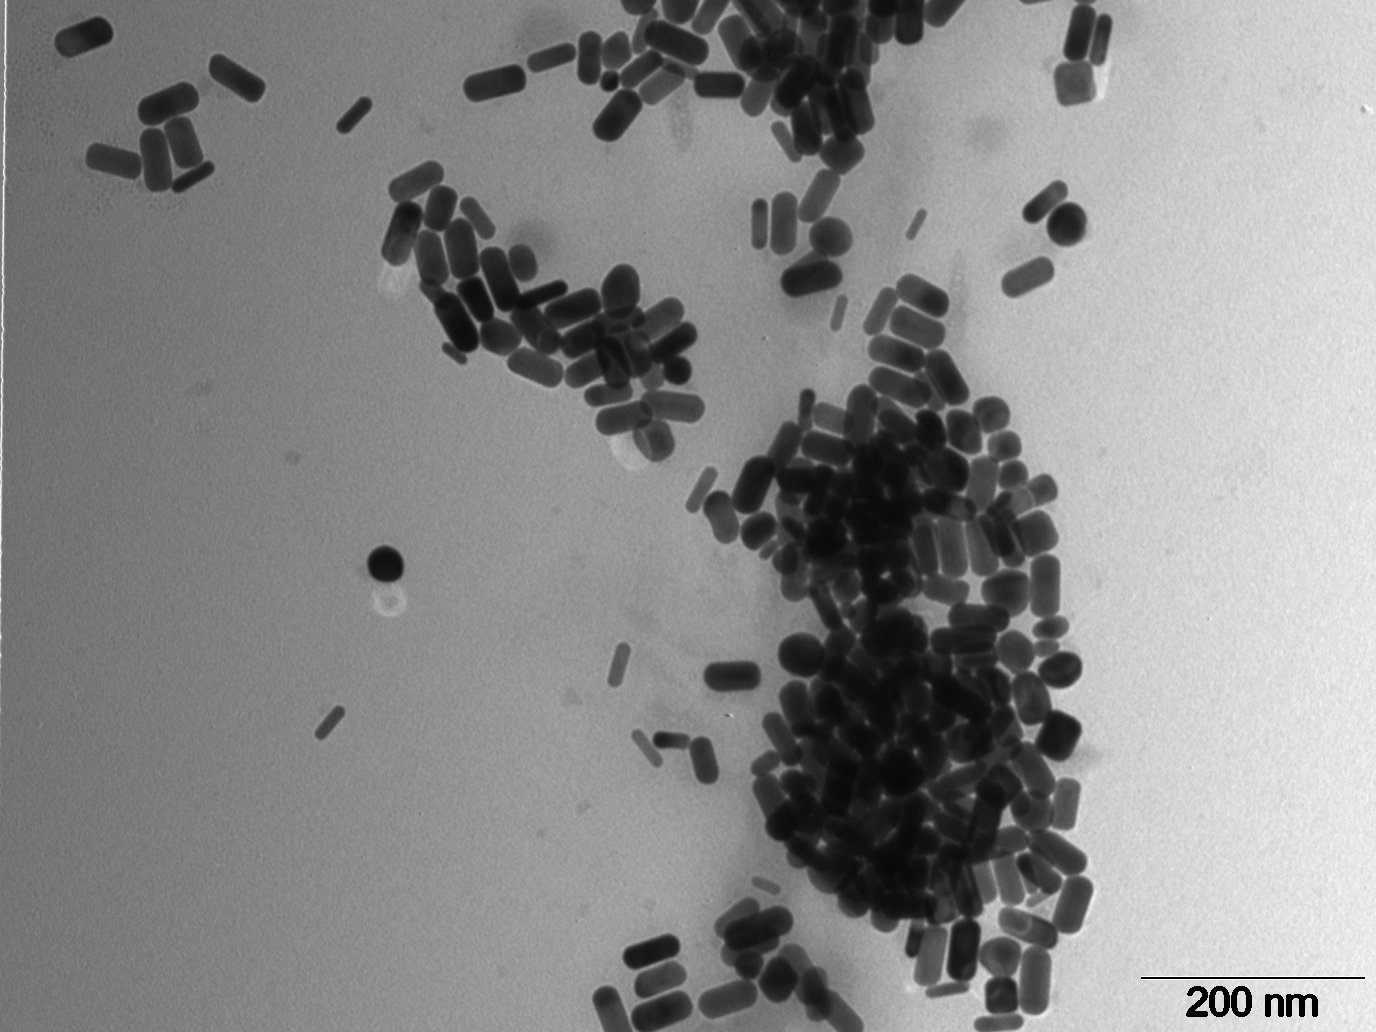
\includegraphics[width=0.48\columnwidth]{Figures/TEM/EO1811.png}
     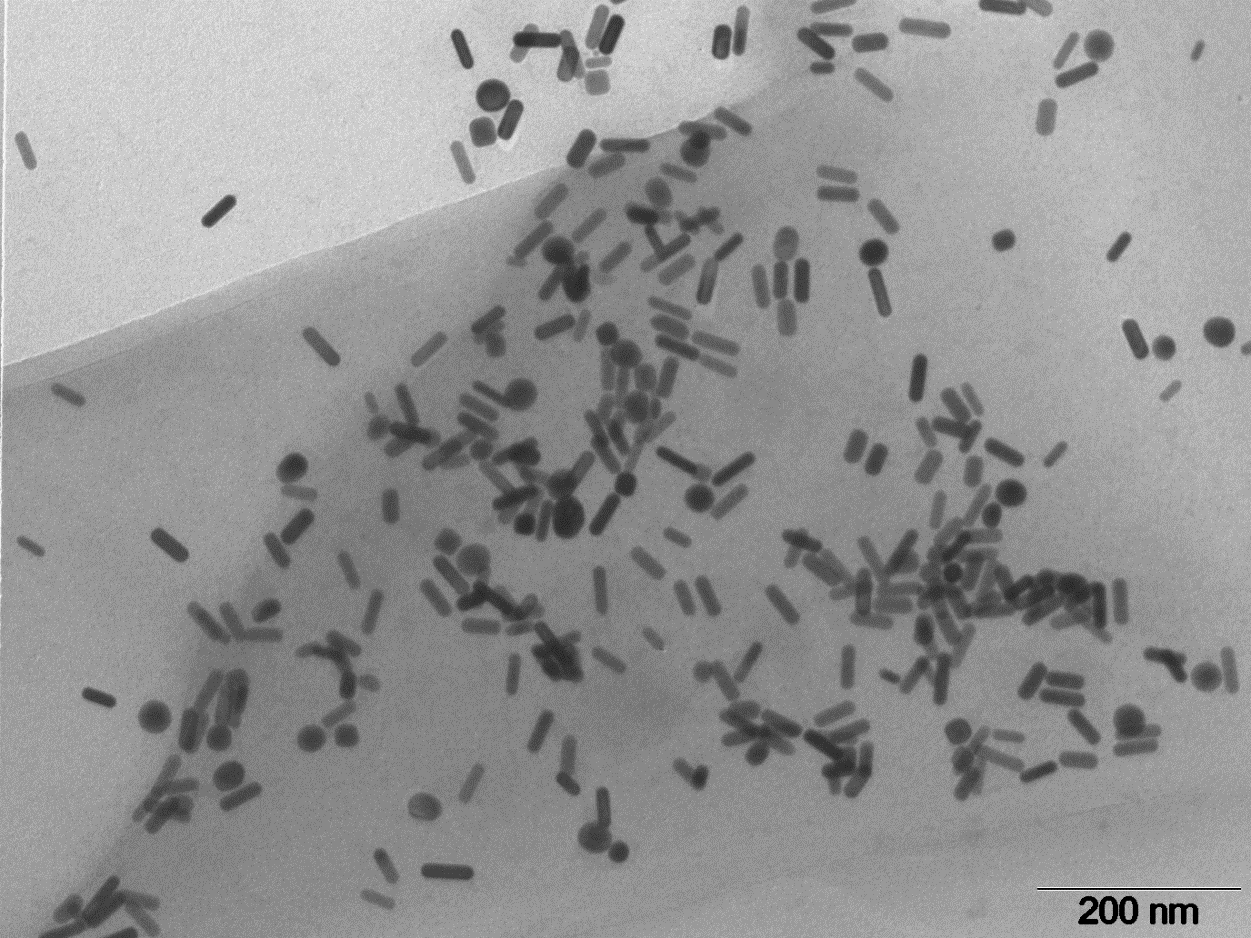
\includegraphics[width=0.48\columnwidth]{Figures/TEM/LB1811.png}
     \includegraphics[width=0.3\columnwidth]{Figures/TEM/L_polydispersity.png}
    \includegraphics[width=0.3\columnwidth]{Figures/TEM/D_polydispersity.png}
    \includegraphics[width=0.3\columnwidth]{Figures/TEM/A_polydispersity.png}
    \caption{Top row, left: Tramsmission Electron Microscope image for the $\overline{A} = 2.1$ Au nanoparticles. Right: TEM image for $\overline{A} = 2.1 $ .Bottom Row distributions for $L$, $D$ and $A$ for the case $\overline{A} = 2.1 $. It is interesting to notice how both the distributions of $L$ and $D$ are Gaussian like, thus leading to an inverse Gaussian distribution for $A$. }
    \label{fig:tem}
\end{figure}


%\begin{figure}
%    \centering
%    \includegraphics[width=0.48\columnwidth]{Figures/TEM/L_polydispersity.png}
%%    \includegraphics[width=0.48\columnwidth]{Figures/TEM/D_polydispersity.png}
 %   \includegraphics[width=0.48\columnwidth]{Figures/TEM/A_polydispersity.png}
 %   \caption{Distributions for $L$, $D$ and $A$ for the case $\langle A=2.1 \rangle$. It is interesting to notice how both the distributions of $L$ and $D$ are Gaussian like, thus leading to an inverse Gaussian distribution for $A$.  }
 %   \label{fig:Polydispersity_TEM}
%\end{figure}

It is interesting to notice that the TEM images, gathered on dried samples for extremely dilute solutions, show a signature of local alignment along the main axes of the nanoparticles. 

The evident polydispersity that characterises the samples stresses the need for an in depth uderstanding of the role that such a parameter plays on the properties of the solution. Such an investigation will be undertaken through a coupled theoretical and computational approach in the following parts of this work. We will address the problem by analysing both polydisperisty as a whole, and thus decoupling all contributions. 


\subsection{Modelling  the Nanoparticles}

The experimental nanorods introduced in the previous section are characterised by a short range repulsive interaction between each other in solution. For this reason, we modelled the particles as spherocylinders, i.e. geometrical shapes consisting of a cylinder of length $L$ and diameter $D$ capped by two hemispheres of diameter $D$, as shown in Fig. \ref{fig:HSC_model}. In the following, we will classify the spherocylinders through their aspect ratio $A = L/D$.

\begin{figure}[!ht]
    \centering
    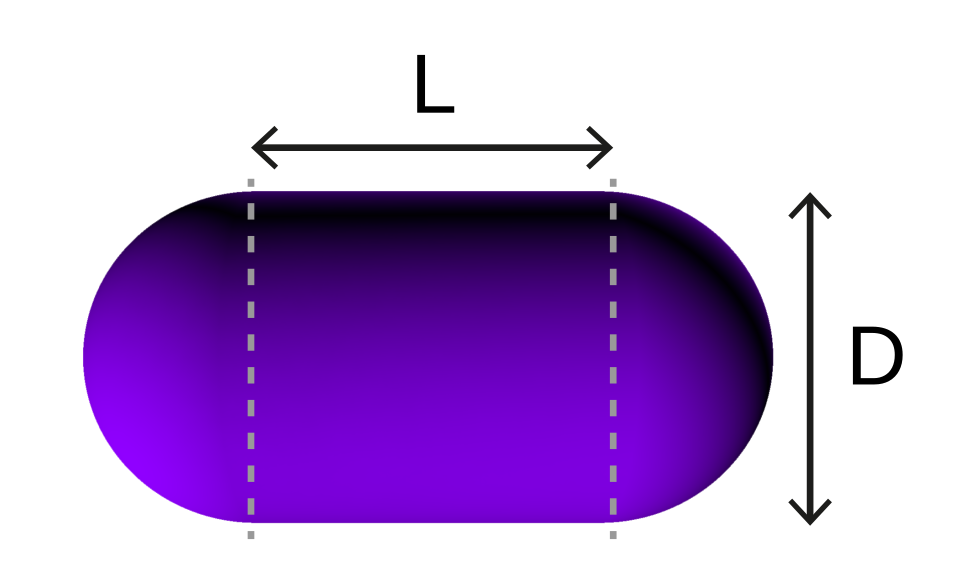
\includegraphics[width=0.25 \columnwidth]{Figures/A1_scheme.png}
    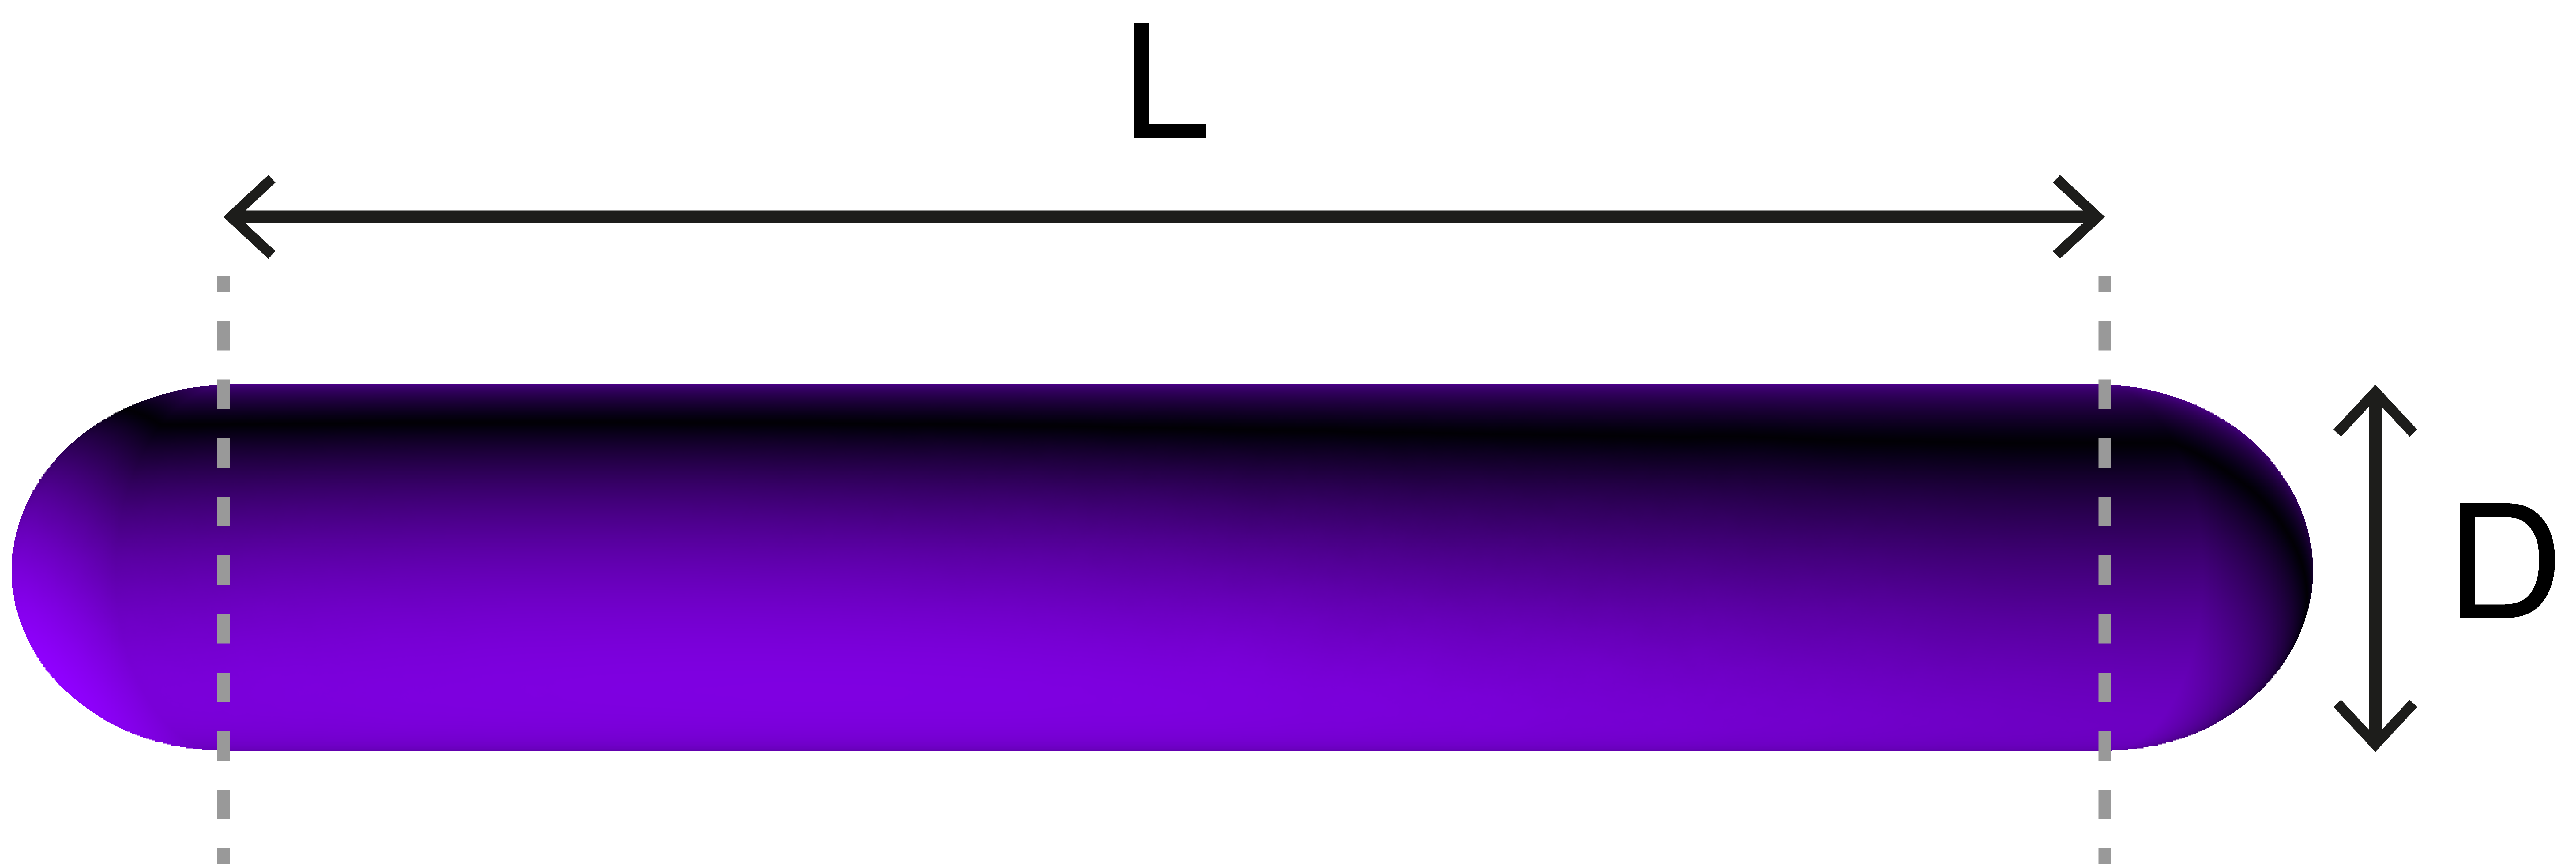
\includegraphics[width=0.45 \columnwidth]{Figures/A5_scheme.png}
    \caption{Representation of a spherocylinder with $A = 1$ (left) and $A = 5$ (right). It is composed by a cylinder of length $L$ and diameter $D$ with two hemispherical ends.}
    \label{fig:HSC_model}
\end{figure}

To obtain information on equilibrium properties of the system, such as the equation of state, local and global characterisations, we perform NPT Monte Carlo simulations for systems composed by $N = 1296$ particles with $A \in [1, 5]$. Inter-particle interaction has been modelled by means of an hard core potential; the estimation of the overlap between particles has been estimated with Vega and Lago algorithm to compute the minimum distance between two rods in three dimensions [cit Vega e Lago].


\begin{comment}
	To estimate such a term, we make use of the Vega and Lago algorithm to compute the minimum distance between two rods in three dimensions. Every MC step  implies the estimation of the overlap between nanoparticles;  every move that would lead to overlap is discarded.
	Equlibration is reached by running the first $1/10$ of the simulation in the canonic ensemble (NVT); then we perform  isothermal-isobaric ensemble simulations (NPT), allowing the system to reach its equilibrium volume.
	 where  the pressure of the system is kept fixed, leaving the volume V of the simulation box free to reach its equilibrium value. 
	Every MC cycle is made by $N$ steps, where $N$ is the total number of particles. One MC step in the NVT ensemble consist of $50\%$ trial random displacement  and $50\%$ random reorientations for each  particle, while in the NPT ensemble the MC moves will consist in  $1/N$ trials in volume change, and all remaining moves will be equally distributed between random displacements and orientations. 
	The volume move consists in an anisotropical change of  one  side of the box chosen randomly. Anysotropic moves are chosen not to introduce any artifcial order in the system (citazione frenkel). 
\end{comment}



\begin{comment}
We introduce the reduced pressure of the system  as $P^* = \beta P v_0$, where $\beta = 1/(k_\mathrm{B} T)$, $k_B$ is the Boltzmann constant, and $v_0$ is the volume of a single particle.
The other quantity that will describe the phase diagram of our system, is the packing fraction, $\phi = v_0 \, \rho = v_0 \, N / V$.
\end{comment}


%In order to rationalise the effect of polydispersity on the phase diagram of functionalized nanoparticles we started by obtaining the equations of state of $N = 1296$ HSCs of various aspect ratios $A = (1, 2, 2.5, 3, 4, 5)$ in low density solution, \textit{i. e.} for reduced pressures $P^* = \beta P v_0 \in [0.01; 1]$.


%Experimentally, each nanoparticle exerts a short range repulsive interaction over the other colloids in solution. In the computational description of the system, such a repulsive term is  modelled through an hard core potential. To estimate such a term, we make use of the Vega and Lago algorithm to compute the minimum distance between two rods in three dimensions. Every MC step  implies the estimation of the overlap between nanoparticles;  every move that would lead to overlap is discarded. 

As introduced in the experimental motivation of the analysis, nanoparticles are affected by a strong polydispersity. In order to quantify their polydispersity, we can introduce the \textbf{P}olydispersity \textbf{I}ndex of a certain quantity $X$ as $PI_X = \Delta X / \overline{X}$, where $\Delta X = PI_X \; \overline{X}$ is the range of a truncated Gaussian centered in $\overline{X}$ and with standard deviation $\sigma_X = {\Delta X}/{ 1.177}$.

Given the elongated nature of the spherocylindrical nanoparticles that are topic of investigation, the system can be subject to a variety of kinds of polydispersity: it can be composed by particles with polydisperse diameter $D$, while their elongation remains unaffected, the opposite can happen - so that the length $L$ is polydisperse and the diameter is monodisperse, or, more coherent with the experimental counterpart, both the quantities can be polydisperse. All those cases introduce a polydispersity over the aspect ratio; nevertheless the choice of the probability distribution defining polydispersity might lead to different equilibrium properties of solutions of polydisperse nanoparticles. To unveil the effect of polydispersity over the equilibrium properties, we  set the starting point of our investigation by computing the monodisperse equation of state ($P^* = \beta P v_0$ as a function of $\phi = v_0 \, N / V$) for nanoparticles with  $A \in [1,5]$ and low packing fractions $\phi < \phi_{N}$, where $\phi_N$ is the isotropic-nematic transition packing fraction.  As a matter of fact $\phi_N=\phi_N(A)$, and the lowest value for $\phi_N$ in the analysed systems is $\phi_N(A)=0.4$ [CITAZIONI, TIPO JACKSON]. We thus perform all of our investigations for $\phi \in (0,0.3]$ (that correspond to reduced pressures $P^* = \beta P v_0 \in [0.01; 1]$). Once determined the monodisperse phase diagram, we perform an in depth investigation over all of the aforementioned combinations for the $L,D$ and $A$ polydispersities. All of the considered combinations for the analysed polydispersities, are shown in figure \ref{fig:Polydispersity_histograms}. 

%As the starting configuration for the simulations is an orthorombic ordered crystalline phase, simulations are performed for $N = 1296$ particles. 




\begin{comment}
Different types of polydispersity have been considered (fig. \ref{fig:poly_hist}):

\begin{itemize}
    \item Monodisperse system as reference;
    
    \item Aspect ratio as a truncated Gaussian:
    \begin{itemize}
    \item $PI_A = 50\% $
    \begin{itemize}
        \item length L as truncated Gaussian and diameter D monodisperse;
        \item length L monodisperse and diameter D as an inverse truncated Gaussian;
    \end{itemize}
    \item $PI_A = 75\% $
    \begin{itemize}
        \item length L as truncated Gaussian and diameter D monodisperse;
        \item length L monodisperse and diameter D as an inverse truncated Gaussian;
    \end{itemize}
        
    \end{itemize}
    
    \item Diameter D as a truncated Gaussian:
    \begin{itemize}
        \item $PI_D = 50\% $
        \begin{itemize}
        \item length L monodisperse and, therefore, A as inverse truncated Gaussian;
        \item length L as truncated Gaussian and, therefore, A as inverse truncated Gaussian.
        \end{itemize}
        \item $PI_D = 75\% $
        \begin{itemize}
        \item length L monodisperse and, therefore, A as inverse truncated Gaussian;
        \item length L as truncated Gaussian and, therefore, A as inverse truncated Gaussian.
        \end{itemize}
    \end{itemize}
    
\end{itemize}

\end{comment}


\begin{figure}[!h]
    \centering
    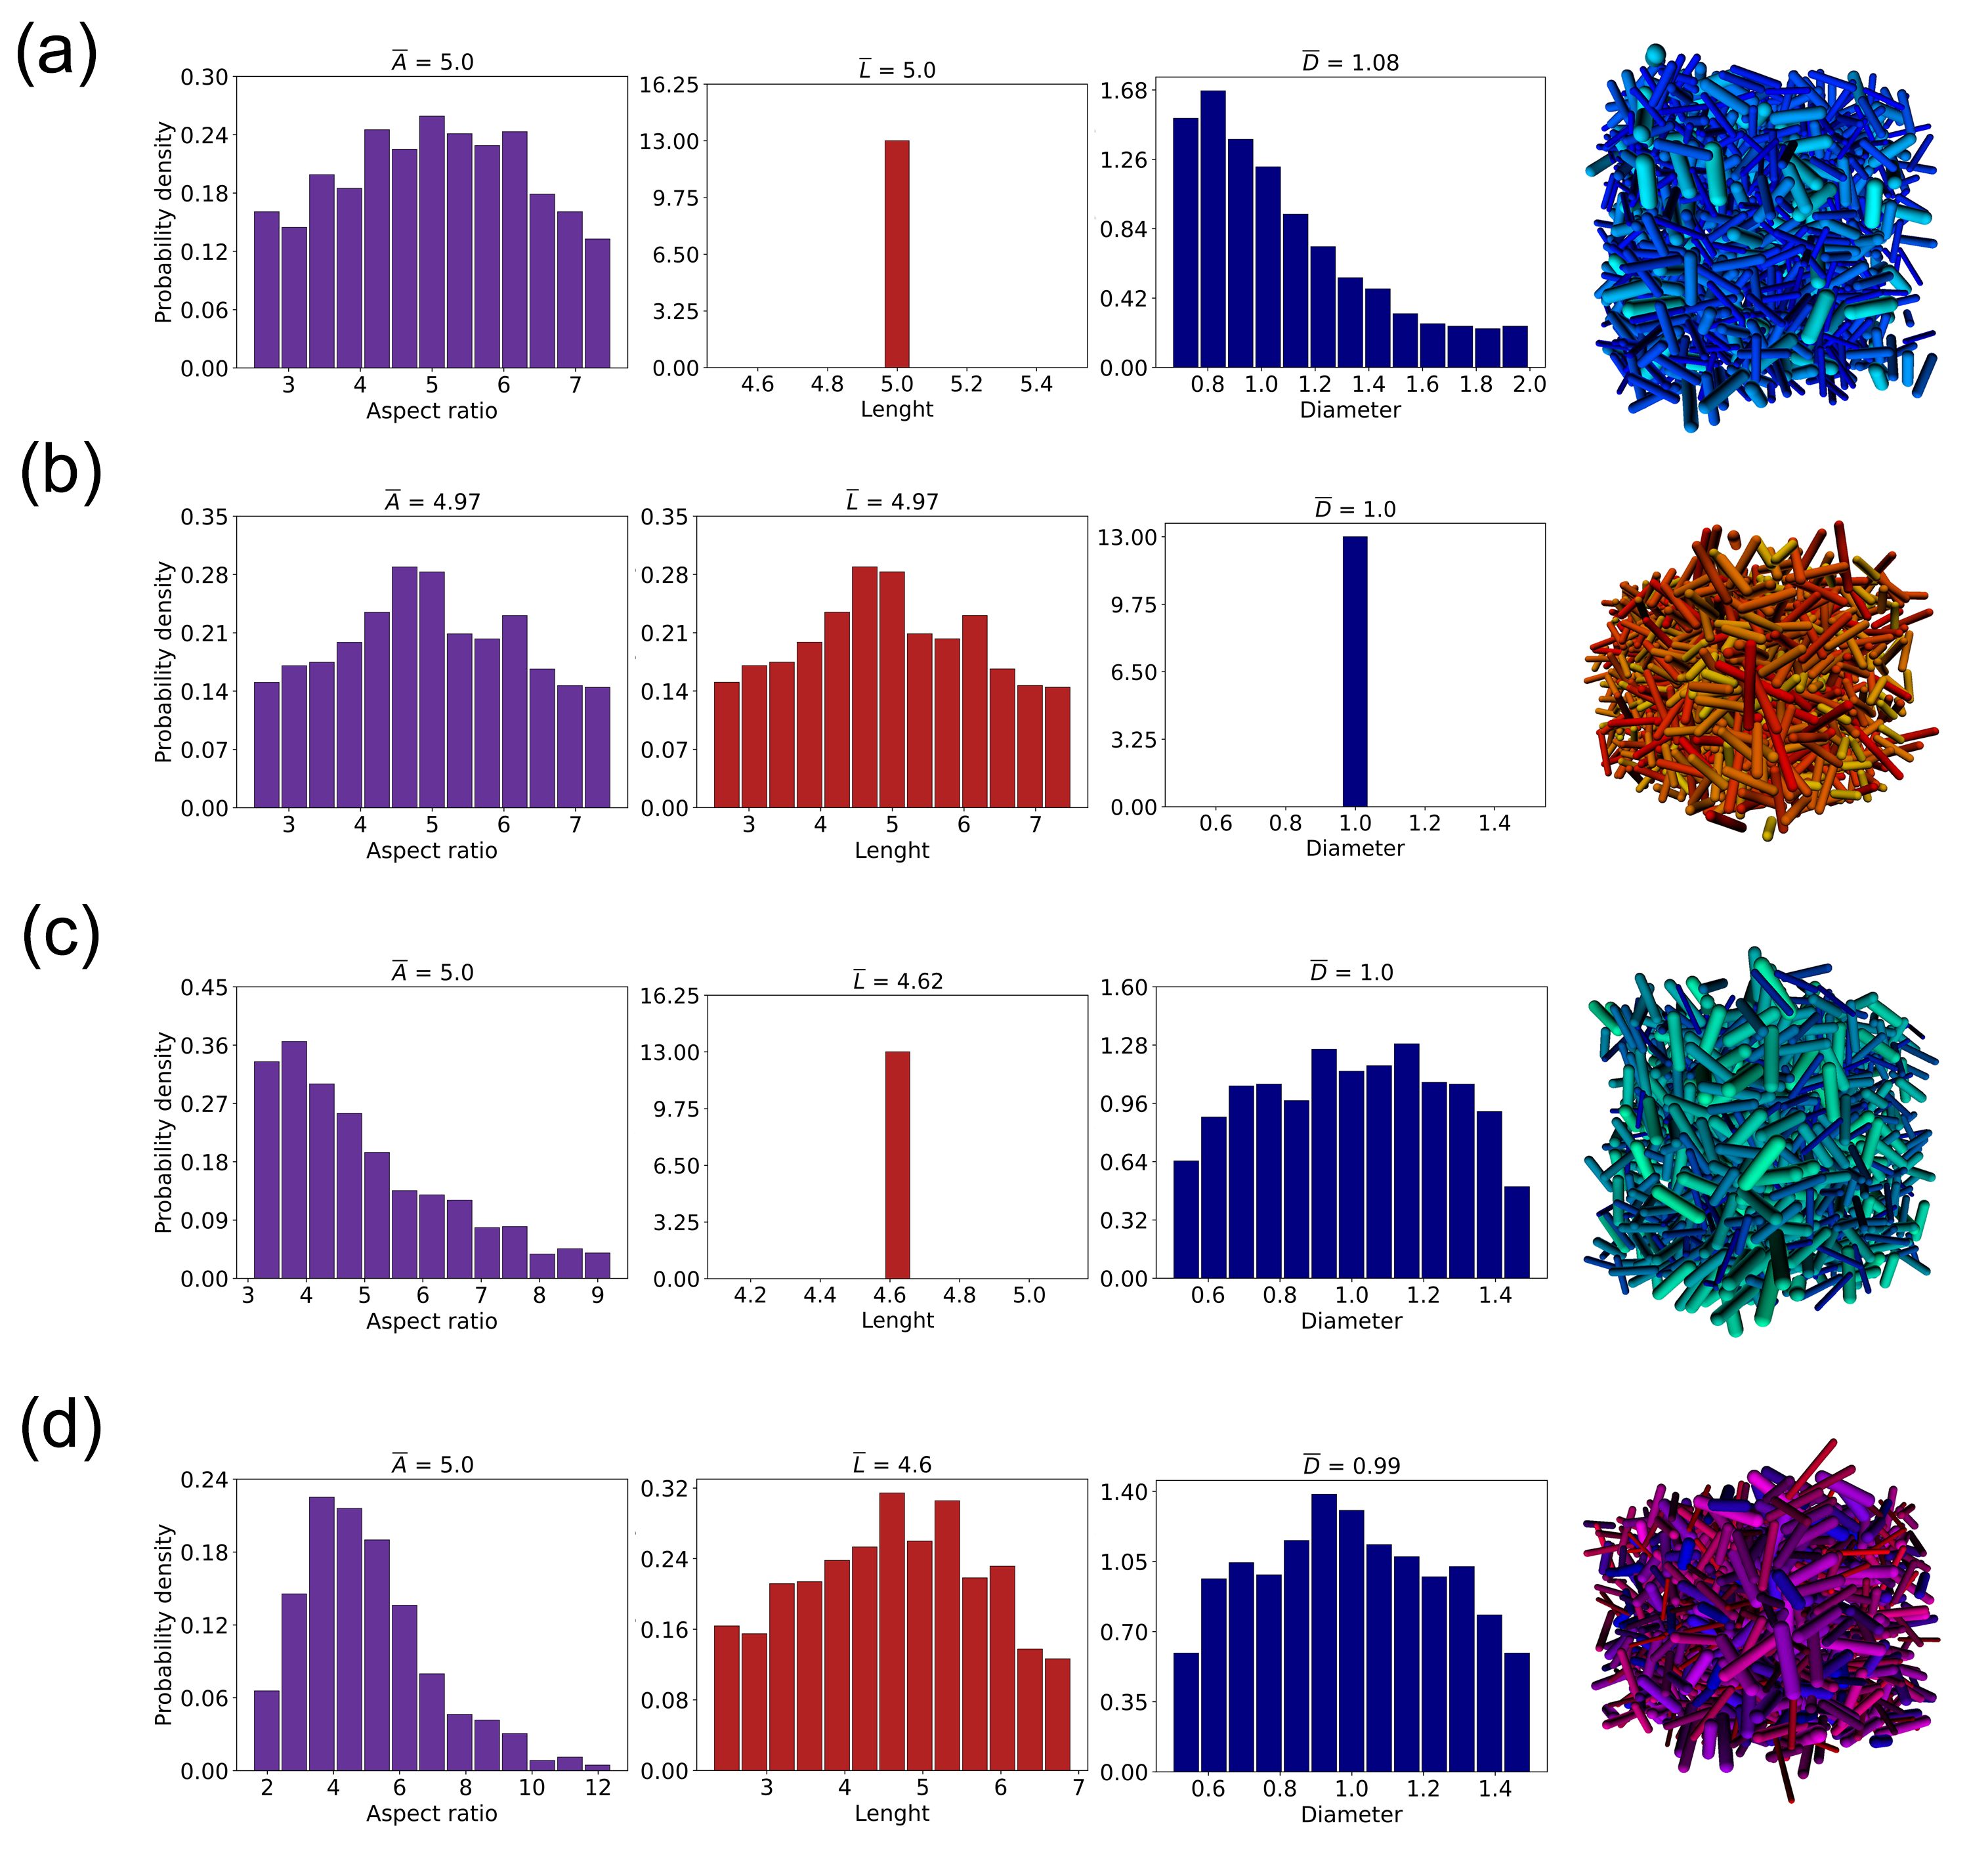
\includegraphics[width=1\columnwidth]{Figures/Polydisp_hist.png}
    %PolyD
    %\includegraphics[width=0.2\columnwidth]{Figures/Polydispersity histograms/PolyD/A_polydispersity.png}
    %\includegraphics[width=0.2\columnwidth]{Figures/Polydispersity histograms/PolyD/L_polydispersity.png}
    %\includegraphics[width=0.2\columnwidth]{Figures/Polydispersity histograms/PolyD/D_polydispersity.png}
    %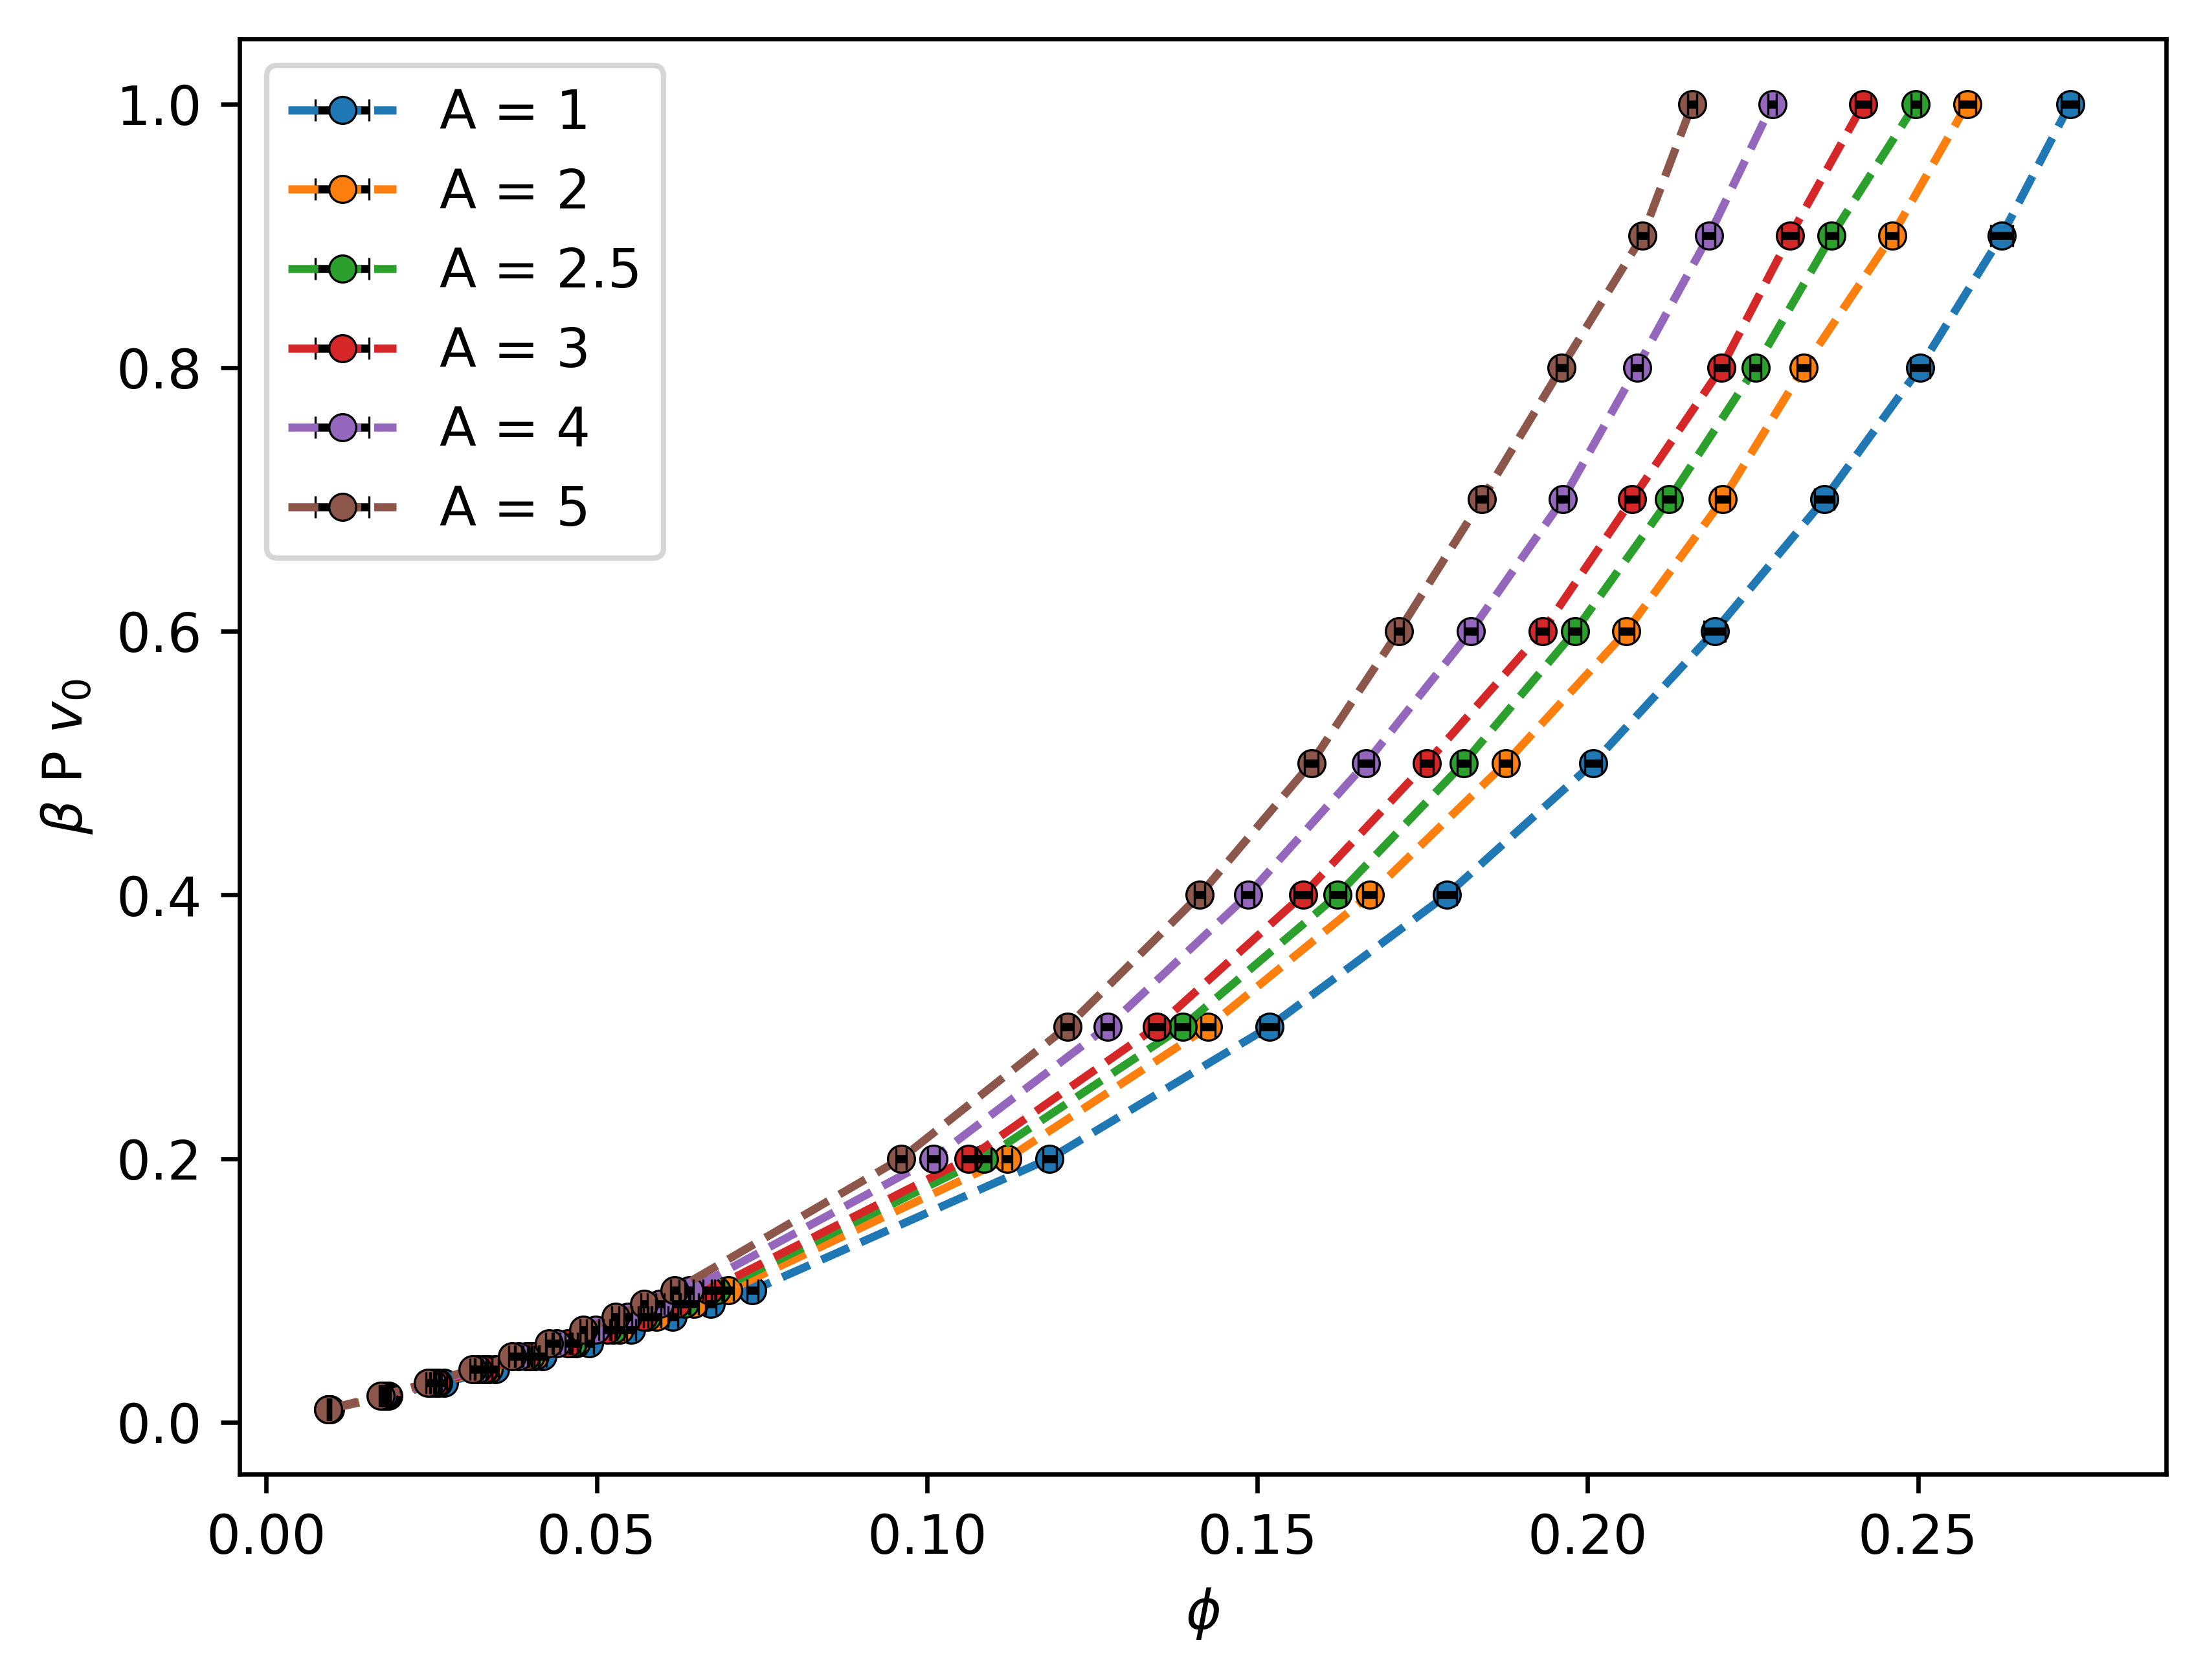
\includegraphics[width=0.2\columnwidth]{Figures/Polydispersity histograms/PolyD/PolyD.png}
    %PolyL
    %\includegraphics[width=0.2\columnwidth]{Figures/Polydispersity histograms/PolyL/A_polydispersity.png}
    %\includegraphics[width=0.2\columnwidth]{Figures/Polydispersity histograms/PolyL/L_polydispersity.png}
    %\includegraphics[width=0.2\columnwidth]{Figures/Polydispersity histograms/PolyL/D_polydispersity.png}
    %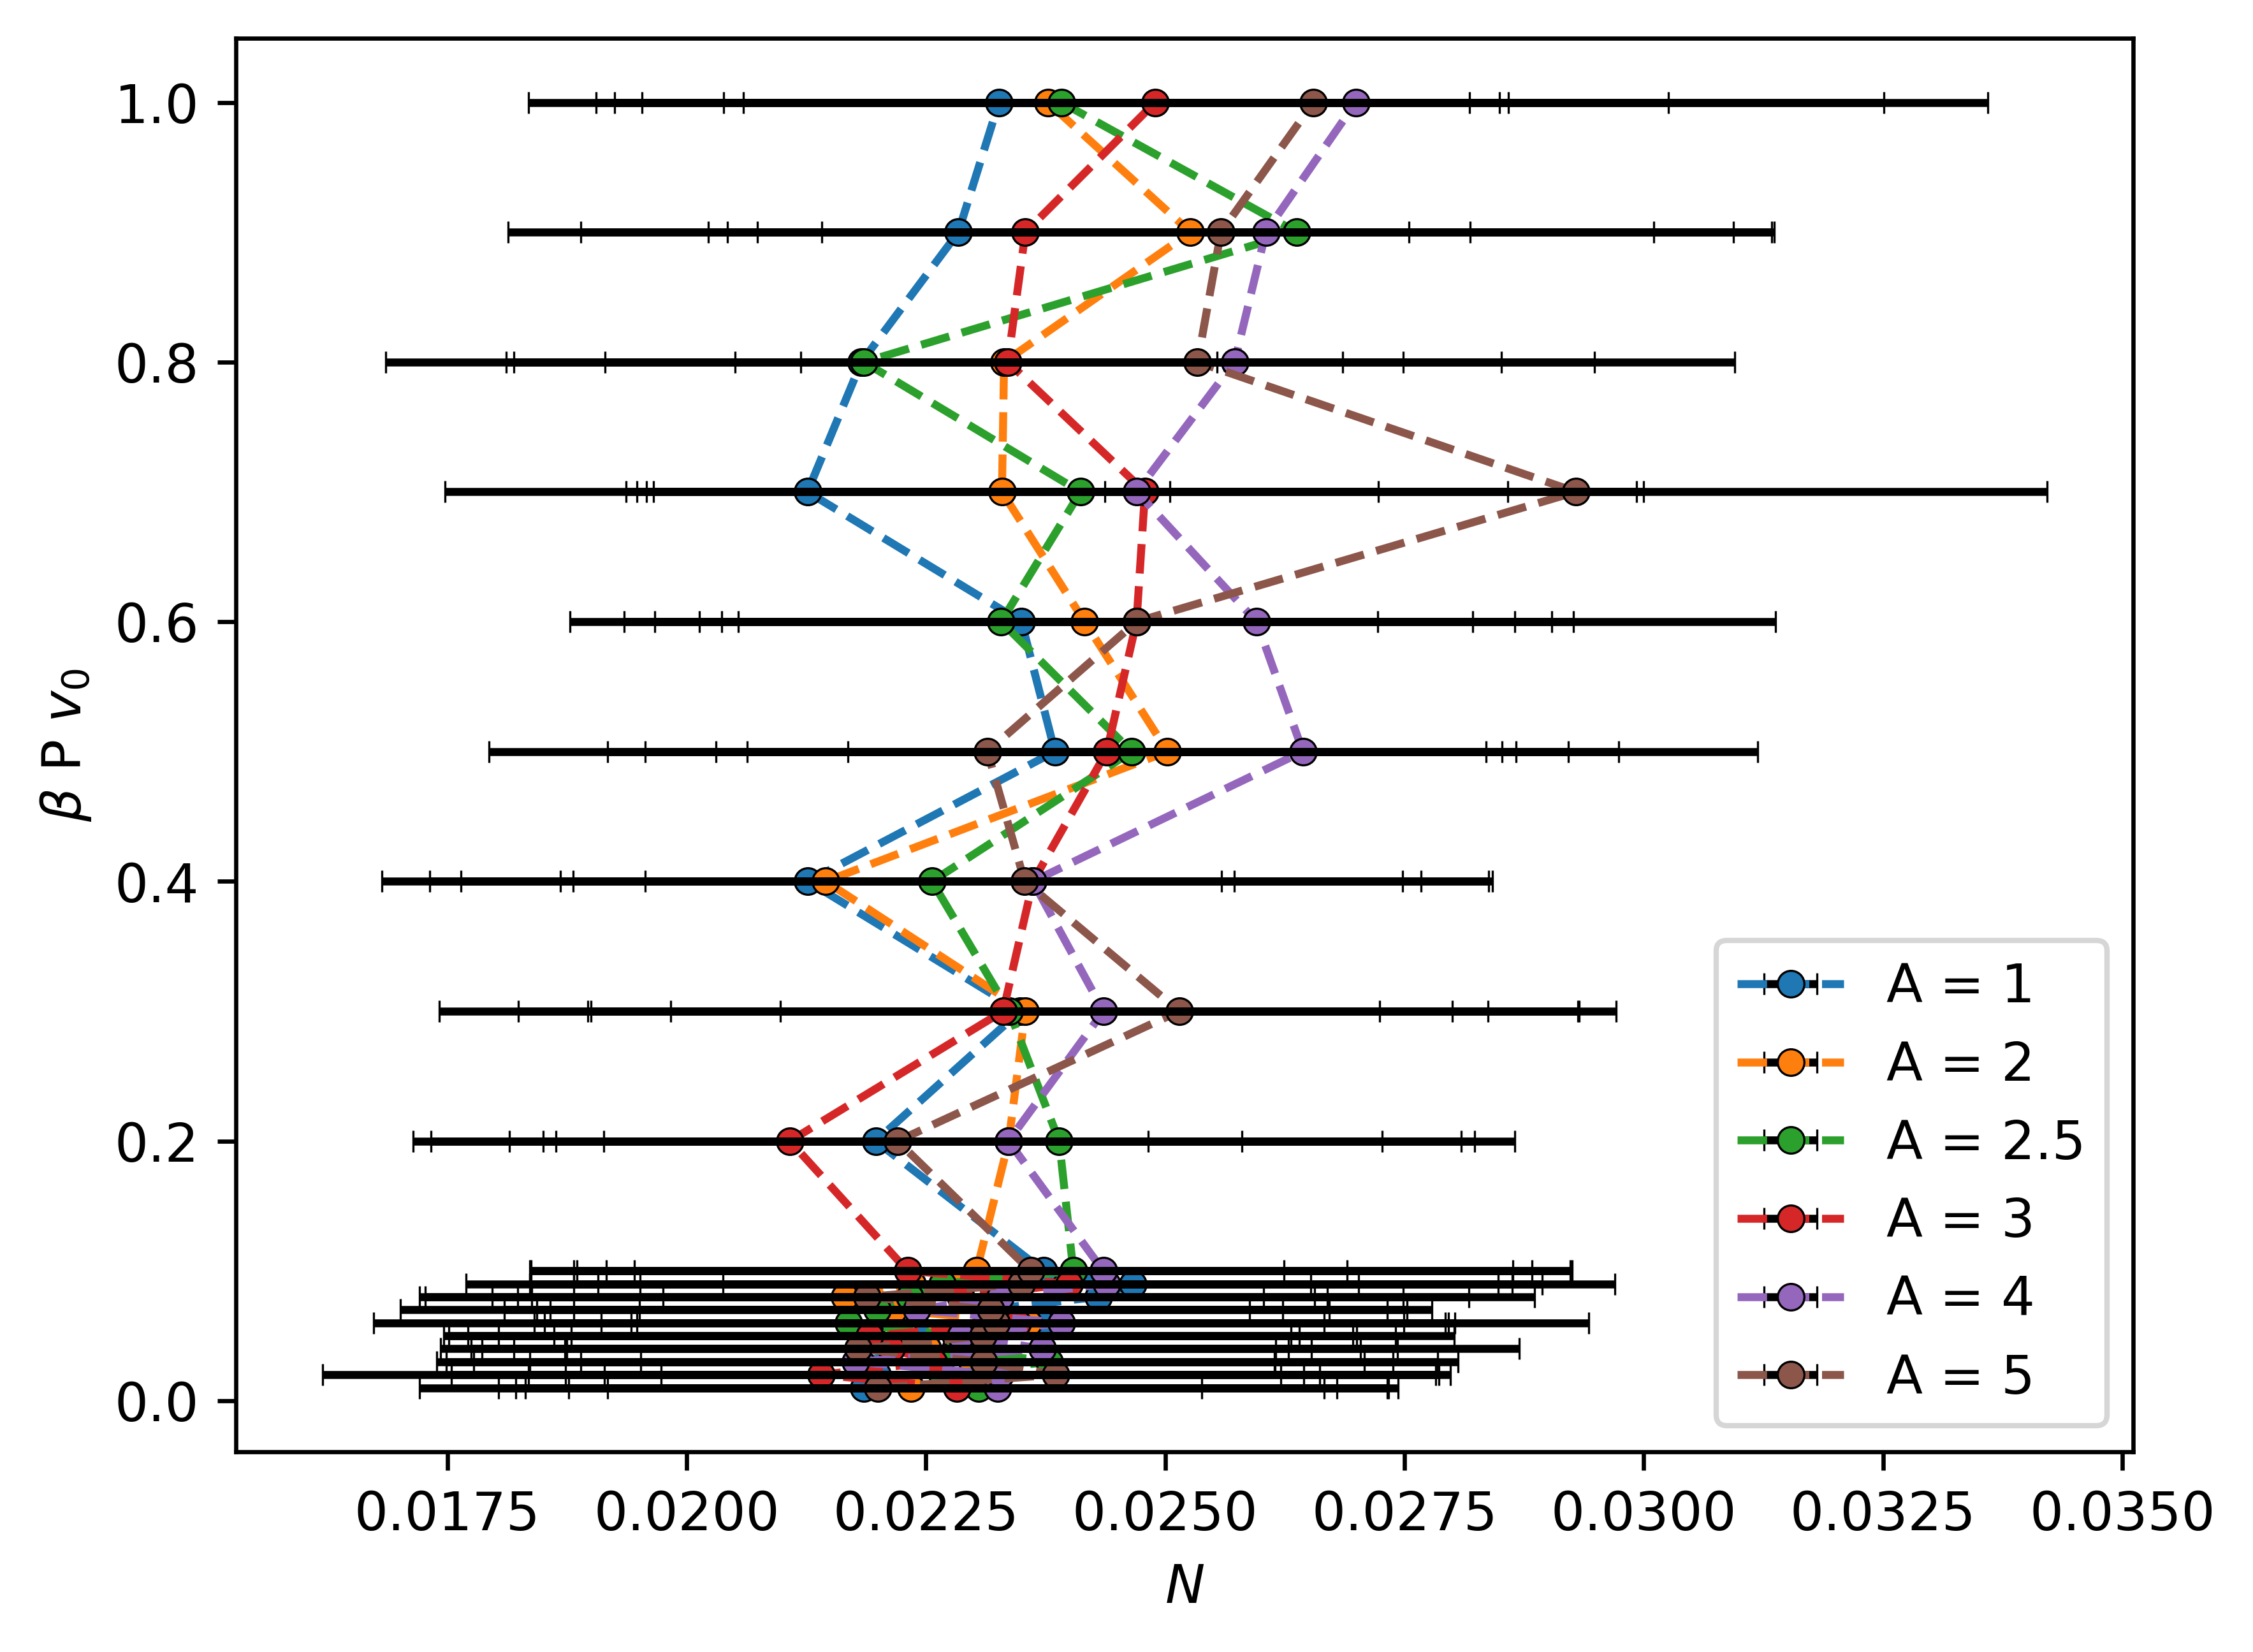
\includegraphics[width=0.2\columnwidth]{Figures/Polydispersity histograms/PolyL/PolyL.png}
    %PolyDGauss
    %\includegraphics[width=0.2\columnwidth]{Figures/Polydispersity histograms/PolyDGauss/A_polydispersity.png}
    %\includegraphics[width=0.2\columnwidth]{Figures/Polydispersity histograms/PolyDGauss/L_polydispersity.png}
    %\includegraphics[width=0.2\columnwidth]{Figures/Polydispersity histograms/PolyDGauss/D_polydispersity.png}
    %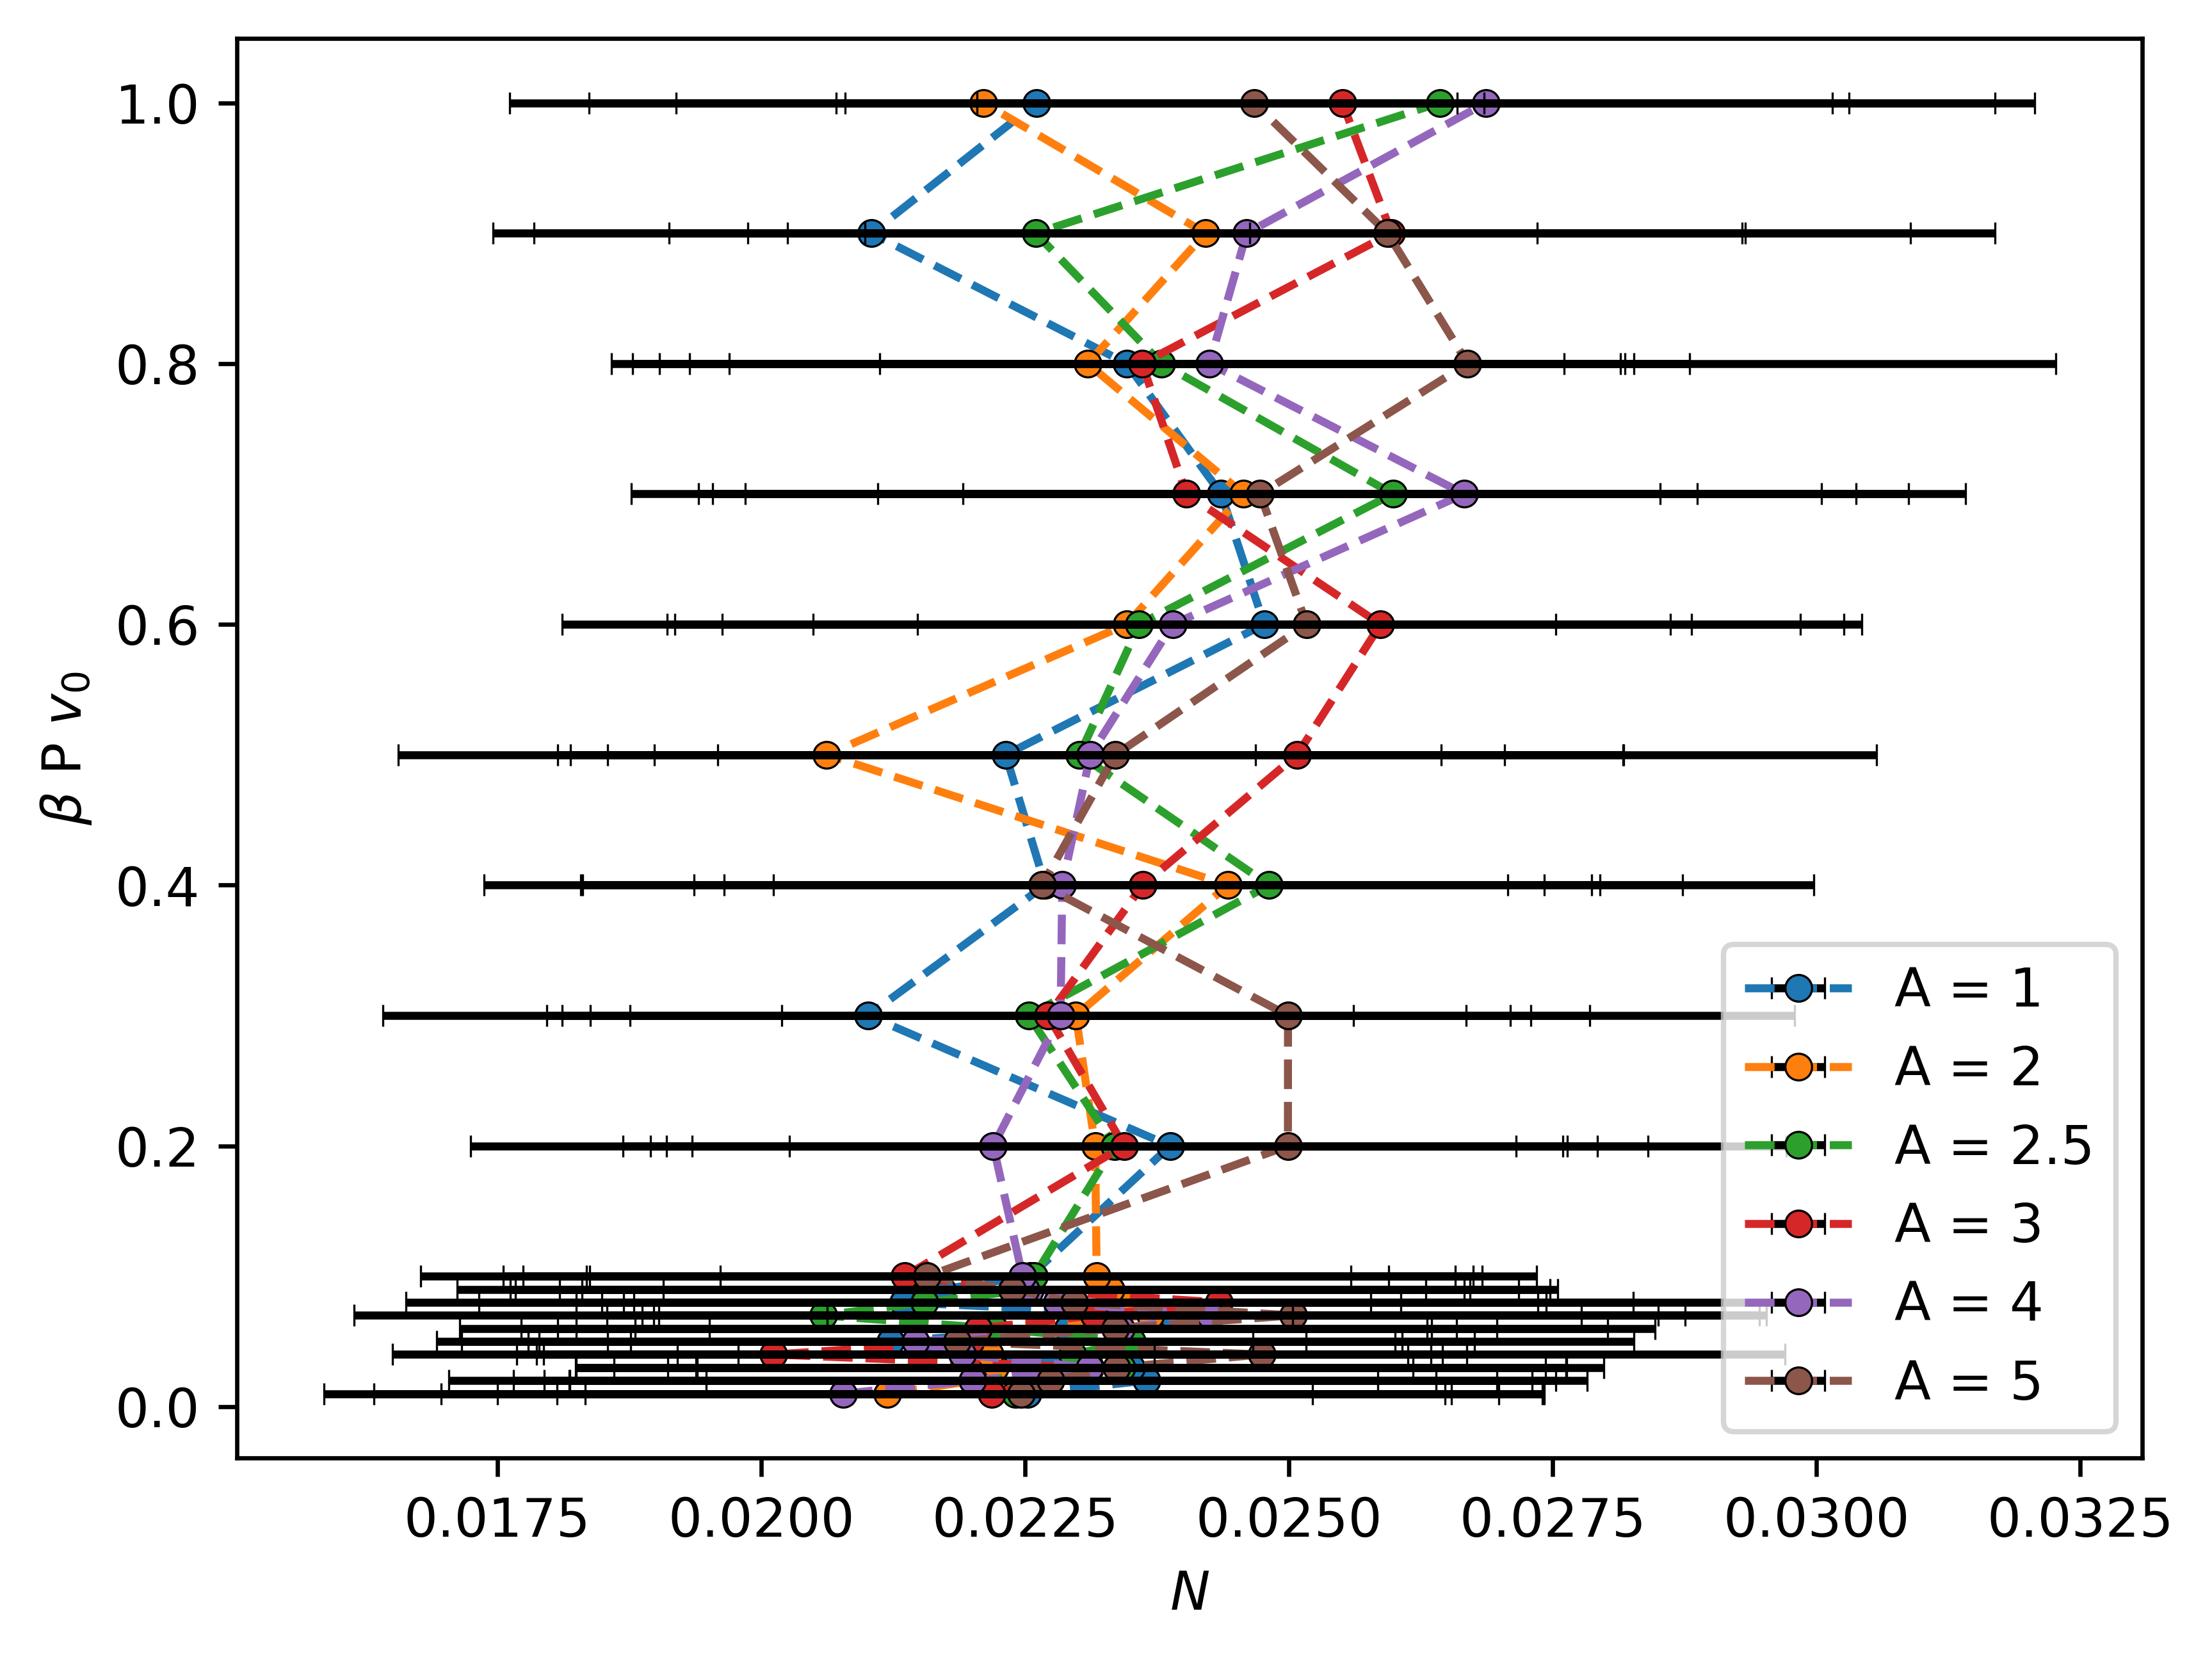
\includegraphics[width=0.2\columnwidth]{Figures/Polydispersity histograms/PolyDGauss/PolyDGauss.png}
    %PolyDLGauss
    %\includegraphics[width=0.2\columnwidth]{Figures/Polydispersity histograms/PolyDLGauss/A_polydispersity.png}
    %\includegraphics[width=0.2\columnwidth]{Figures/Polydispersity histograms/PolyDLGauss/L_polydispersity.png}
    %\includegraphics[width=0.2\columnwidth]{Figures/Polydispersity histograms/PolyDLGauss/D_polydispersity.png}
    %\includegraphics[width=0.2\columnwidth]{Figures/Polydispersity histograms/PolyDLGauss/polyDLGauss.png}
    
    \caption{Histograms of the types of system polydispersities analysed in this work (only $A = 5$ represented here). Each type of system has been studied with both $50 \%$ and $75 \%$ of Polidispersity Index. (a) Polydisperse D: the distribution of the aspect ratio is a truncated Gaussian while the length is monodisperse, therefore the diameter is represented as an inverse truncated Gaussian. (b) Polydisperse L: the aspect ratio and the length of the particles are truncated Gaussians while the diameter is monodisperse. (c) Polydisperse D Gauss: the diameter follows a truncated Gaussian distribution while the length is monodisperse, therefore the aspect ratio is the inverse of a truncated Gaussian. (d) Polydisperse D L Gauss: both the length and the diameter of the particles are truncated Gaussians, therefore the aspect ratio is the inverse of a truncated Gaussian.}
    \label{fig:Polydispersity_histograms}
\end{figure}


\subsection{Theory} \label{sec:Theory}
Simulations will be coupled and compared with theoretical predictions. We can assume that in the isotropic phase the free energy of the system can be written as [citazioni]:

\begin{equation}
	F = F^{id} + F^{or} + F^{excl}
\end{equation}

where the first two terms account for the ideal gas free energy ($F^{id}$) and for the entropy due to large scale orientational order ($F^{or}$), while the third is the excluded-volume contribution. 


To estimate the excess term, we make use of the Parson-Lee approach for the excluded volume term [citazioni] that extends Onsager's work [cit Onsager] by including higher-body terms of the virial expansion. Within such an approximation, the excess free energy becomes 

\begin{equation}
\frac{\beta F_{excl}}{N}  = \frac{\phi \, \eta(\phi)}{2 \, \overline{v_{0}}} \iint v_{excl}(\gamma[\Omega_1, \Omega_2]) f(\Omega_1)f(\Omega_2) d\Omega_1 d\Omega_2    
\end{equation}

where $\eta(\phi) = \frac{1}{4} \frac{4 - 3\phi}{(1 - \phi)^2}$ is the Parson-lee factor, $v_{exc}$ is the mutual excluded volume between two spherocylinders with respective orientations $\Omega_1$ and $\Omega_2$, $f(\Omega)$ is the orientational distribution function, and $\overline{v_0}$ is the average volume of the particles in the system.

The total free energy per particle can be explicitated as:
\begin{equation}
    \frac{\beta F}{N} = \ln(\Lambda^3 \rho) - 1 + \int f(\Omega) \ln(4 \pi f(\Omega)) d \Omega + \frac{\phi \, \eta(\phi)}{2 \, \overline{v_{0}}} \iint v_{excl} (\Omega_1, \Omega_2) f(\Omega_1)f(\Omega_2) d\Omega_1 d\Omega_2
\end{equation}

where $\Lambda$ is the de Broglie thermal wavelength and $\rho = N/V$ is the number density. The integral in the last term corresponds to the average excluded volume $\overline{v_{excl}}$ between the particles in the system and its calculation depends on the size distribution of the particles in the system and on their mutual orientation. Its computation, along with the estimation of the average particle volume, is explained in detail in the SI.

The reduced pressure $P^*$ of the system can be obtained from the free energy as:

\begin{equation}
    P^* =  P^*_{id} - \beta \, \overline{v_0} \frac{\partial F_{excl}}{\partial V} \rvert _{N, T}  = \phi - N \beta \, \overline{v_0} \frac{\overline{v_{excl}}}{8 \, \overline{v_0}} \frac{\partial}{\partial V} \left( \phi \frac{4 - 3 \phi}{(1 - \phi)^2} \right) \nonumber = \phi + \frac{\overline{v_{excl}}}{4 \, \overline{v_0}} \phi^2 \frac{2 - \phi}{(1 - \phi)^3} \label{ParsonLee}
\end{equation}


\subsection{Equation of state}

As a reference starting point we computed the equation of state of the monodisperse system as a function of the elongation, \textit{i. e.} the aspect ratio $A$ of the particles. The results are coherent with the previous studies found in literature (citazioni FRENKEL in particolare, jackson): the more the particles are elongated, the less the system is compressible.


To assess the role of polydispersity and the contribution on the compressibility of polydispersity on length and diameter separately, we performed simulations for  all of the combinations reported in Fig. \ref{fig:Polydispersity_histograms}, keeping fixed the mean aspect ratio $A$ of the system to the monodisperse counterpart.

In figure \ref{fig:EOS_HSC_comparison} are reported two out of all of the analysed cases for sake of clarity.

\begin{figure}[!h]
    \centering
    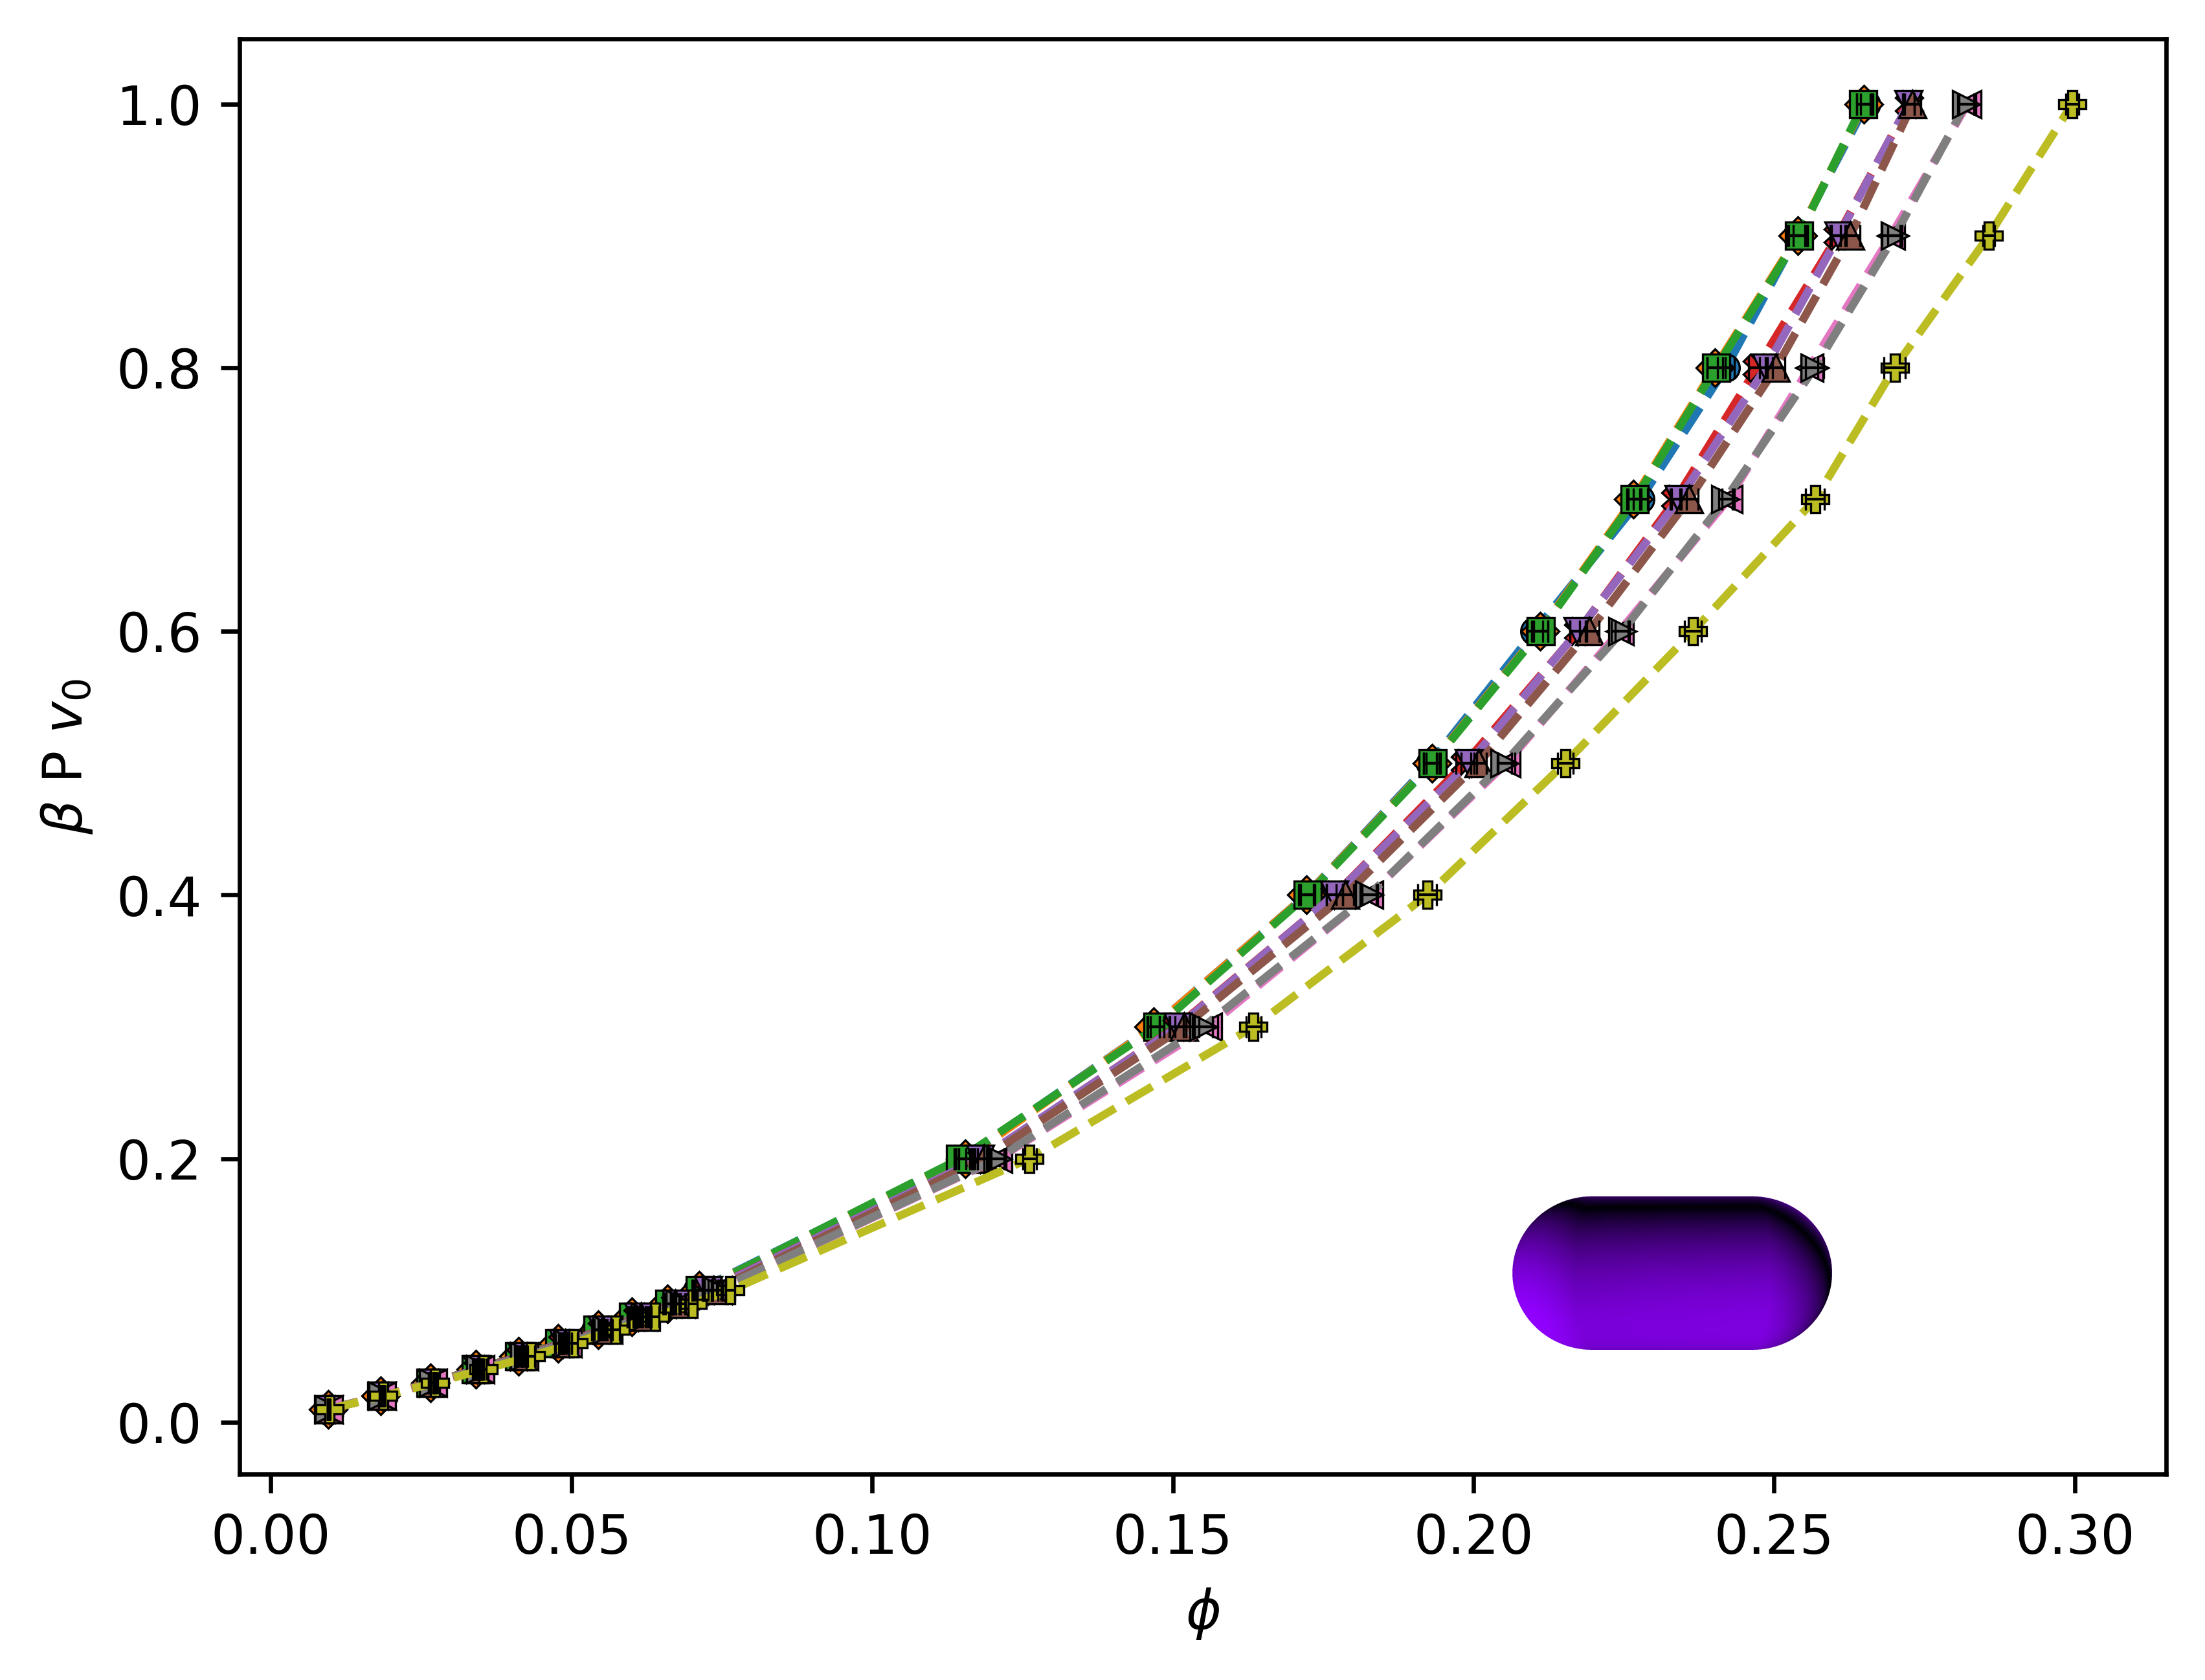
\includegraphics[width=0.45 \columnwidth]{Figures/EOS_A1.png}
    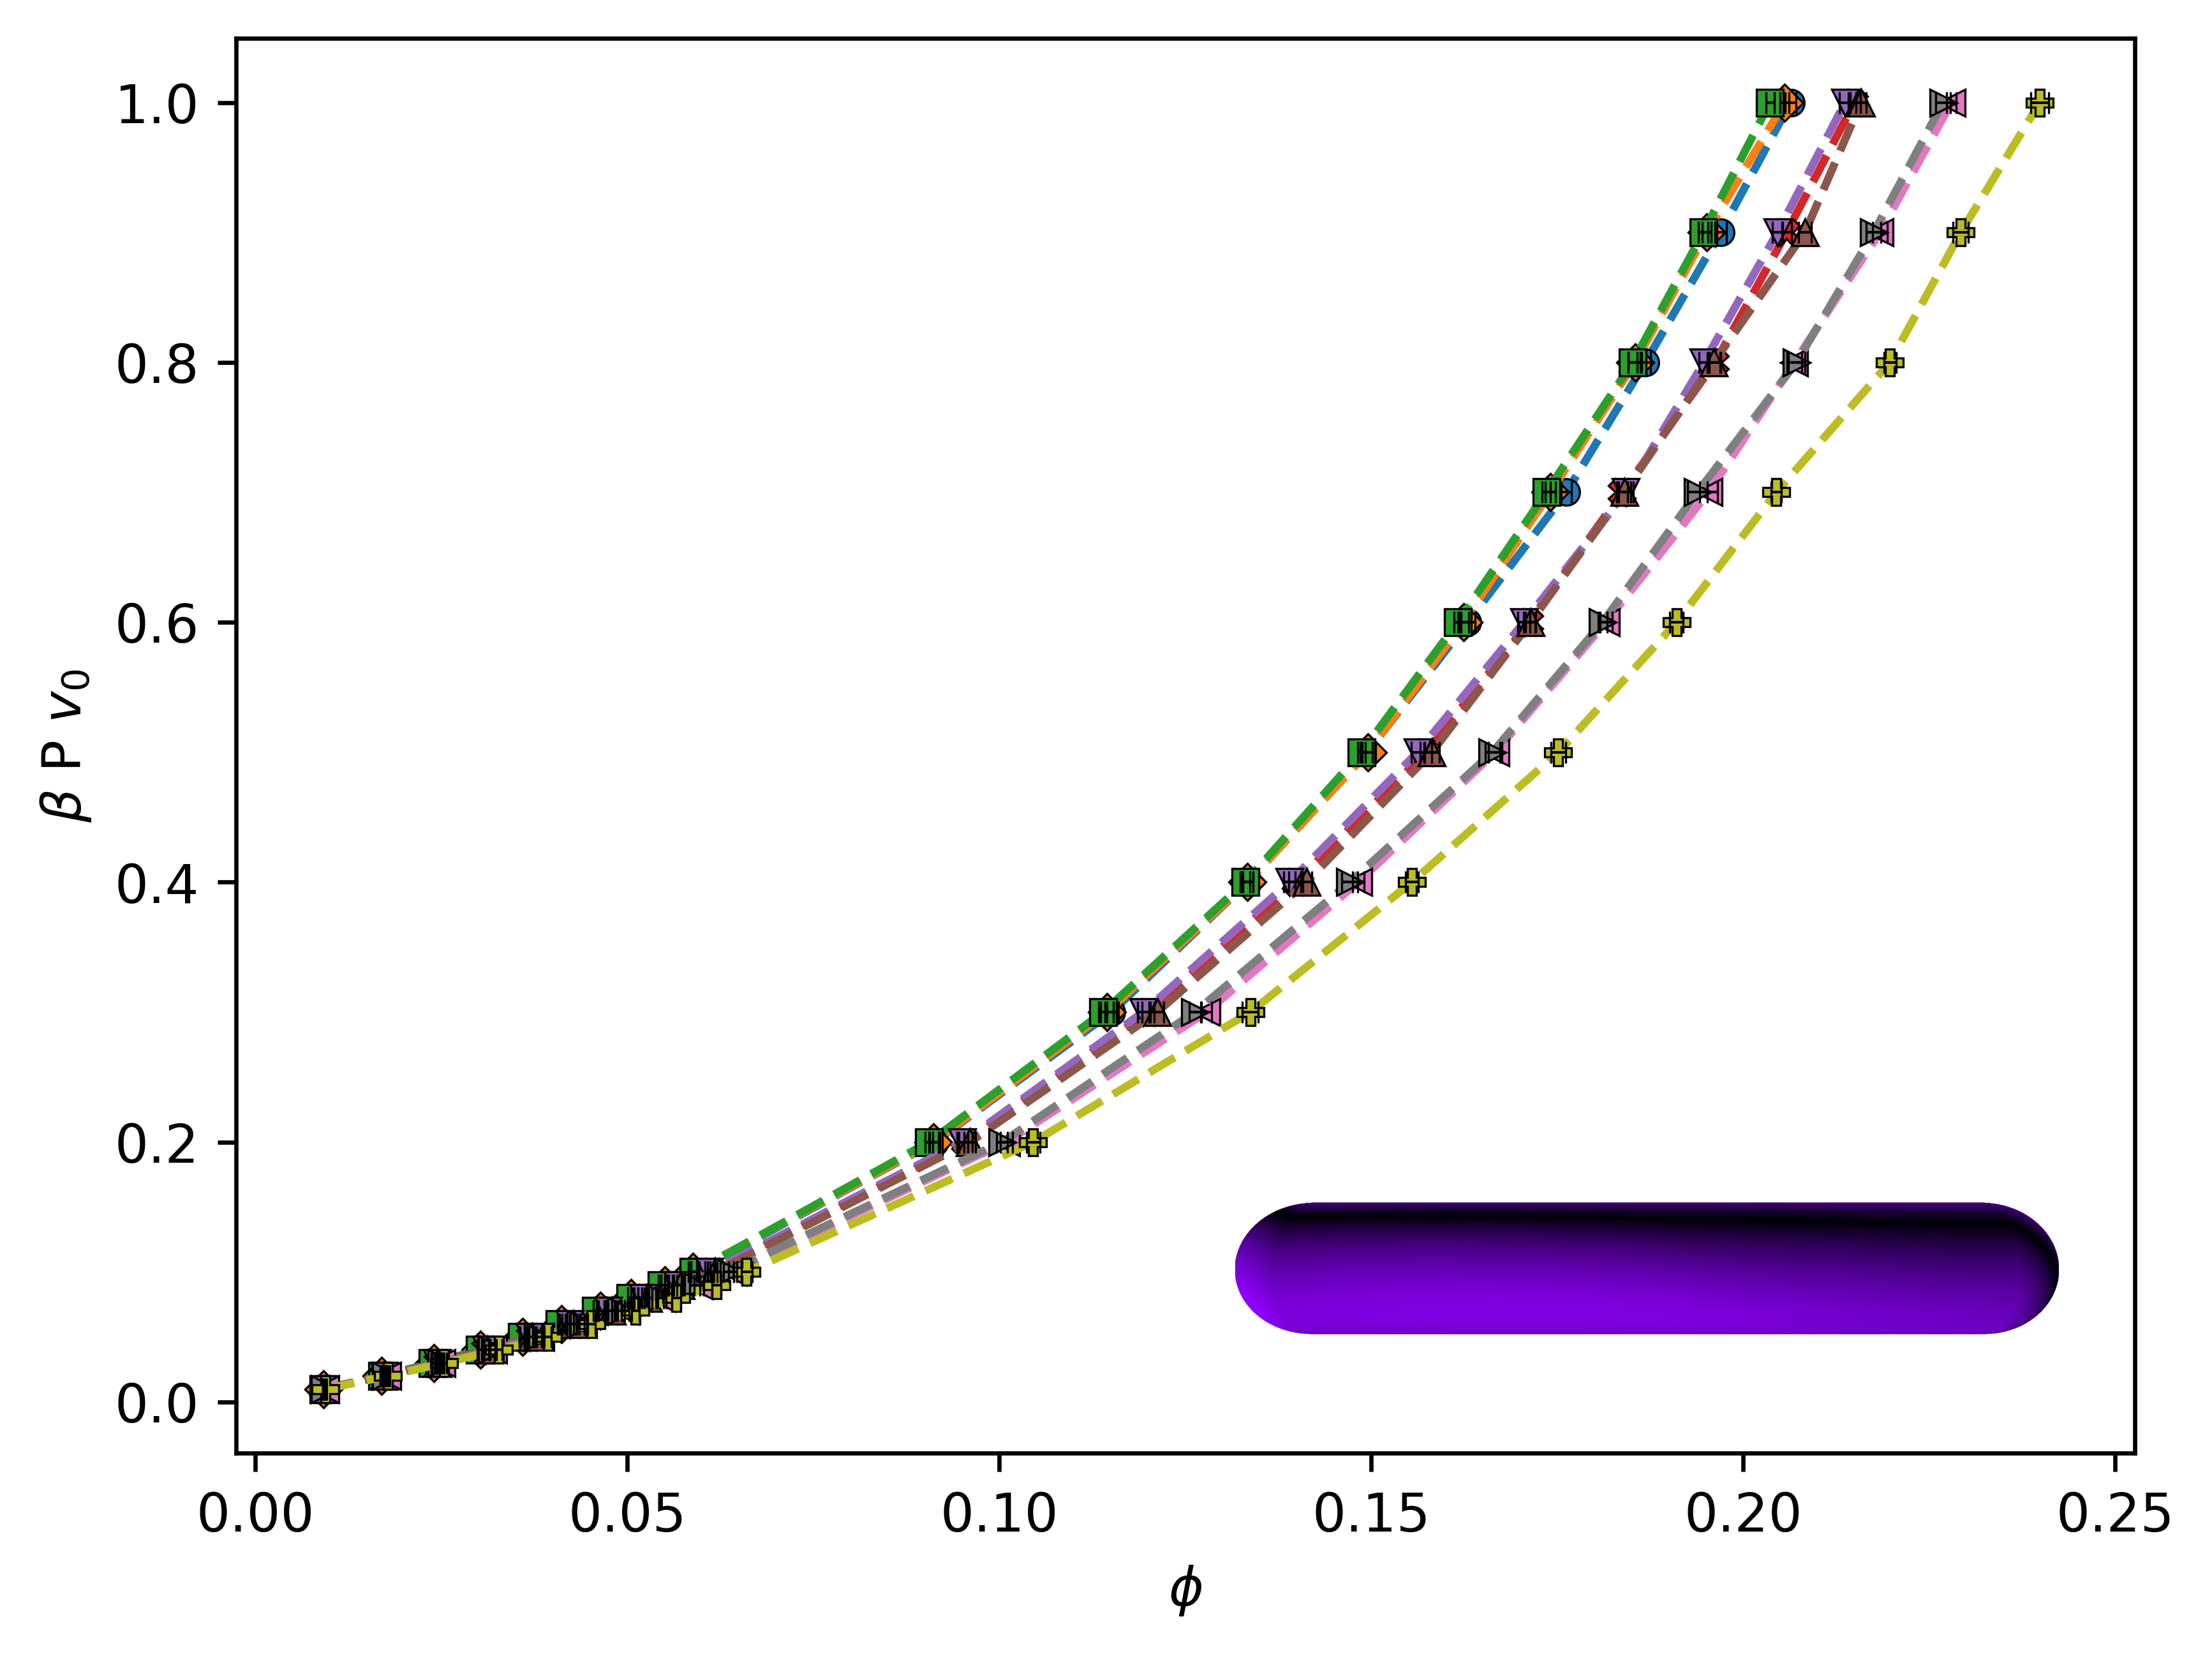
\includegraphics[width=0.45 \columnwidth]{Figures/EOS_A5.png}
    \caption{Equation of state of the systems analysed in this work for $A = 1$ (right) and $A = 5$ (left): monodisperse (circles), polydisperse L (diamonds), polydisperse L 75 \% (squares), Gauss polydisperse D (x symbols), Gauss polydisperse D and L (downward triangles), polydisperse D (upward triangles), Gauss polydisperse D 75 \% (leftward trinagles), Gauss polydisperse D and L 75 \% (rightward triangles), and polydisperse D 75 \% (plus symbols).  (Aggiungere un inset con la magnification in alto a sinistra?)}
    \label{fig:EOS_HSC_comparison}
\end{figure}

We can immediately notice that any of the introduced polydispersities in the length $L$ of the particles (up to $75\%$) do not affect the low density EOS of the solution. On the other hand, a polydispersity on the diameter $D$ results in a huge enhancement of compressibility of the system: the system reaches a higher equilibrium packing fraction $\phi$ at the same reduced pressure $P^*$ and the resulting EOS seems to be dependent on the particular polydispersity distribution of the diameters.

Given the low packing fractions analysed, and being the system below the isotropic nematic transition, the discrepancy in the roles played by a polydispersity either in $D$ or in $L$, might be linked to a rise of  self-organisation within the system. To investigate whether this could be the case, we analysed both local and global properties of the solutions, by computing the  radial pair distribution function $g(r)$, the orientational radial distribution function $g_2(r)$, and the nematic order parameter $S$.  The results, reported in detail in the SI, show no sign of orientational or spatial ordering in the system with no noticeable differences between the monodisperse and the polydisperse cases for a given aspect ratio.




\subsection{Theory comparison}
In this section we report the comparison between predicted EOS predicted through the theoretical approach defined in section THEORY, and the computational results. 
The mean field theory is able to qualitatively reproduce the EOS, for all of the considered cases. As happened in the simulations, introducing a polydispersity in $L$ does not affect in any way the EOS, while all of the considered polydispersities in $D$ change the compressibility of the corresponding monodisperse case. In addition, the effect on the compressibility of the diameter polydispersity seems to be linked to their distribution (graphical comparison in SI).


Strikingly, while the numerical comparison between EOS obtained through simulations and theoretically is only qualitative, the deviation between the monodisperse and polydisperse predicted packing fractions for all of the analysed cases is quantitative, as can be see in figure \ref{fig:DeltaP_P}. 

\begin{figure}[!h]
    \centering
    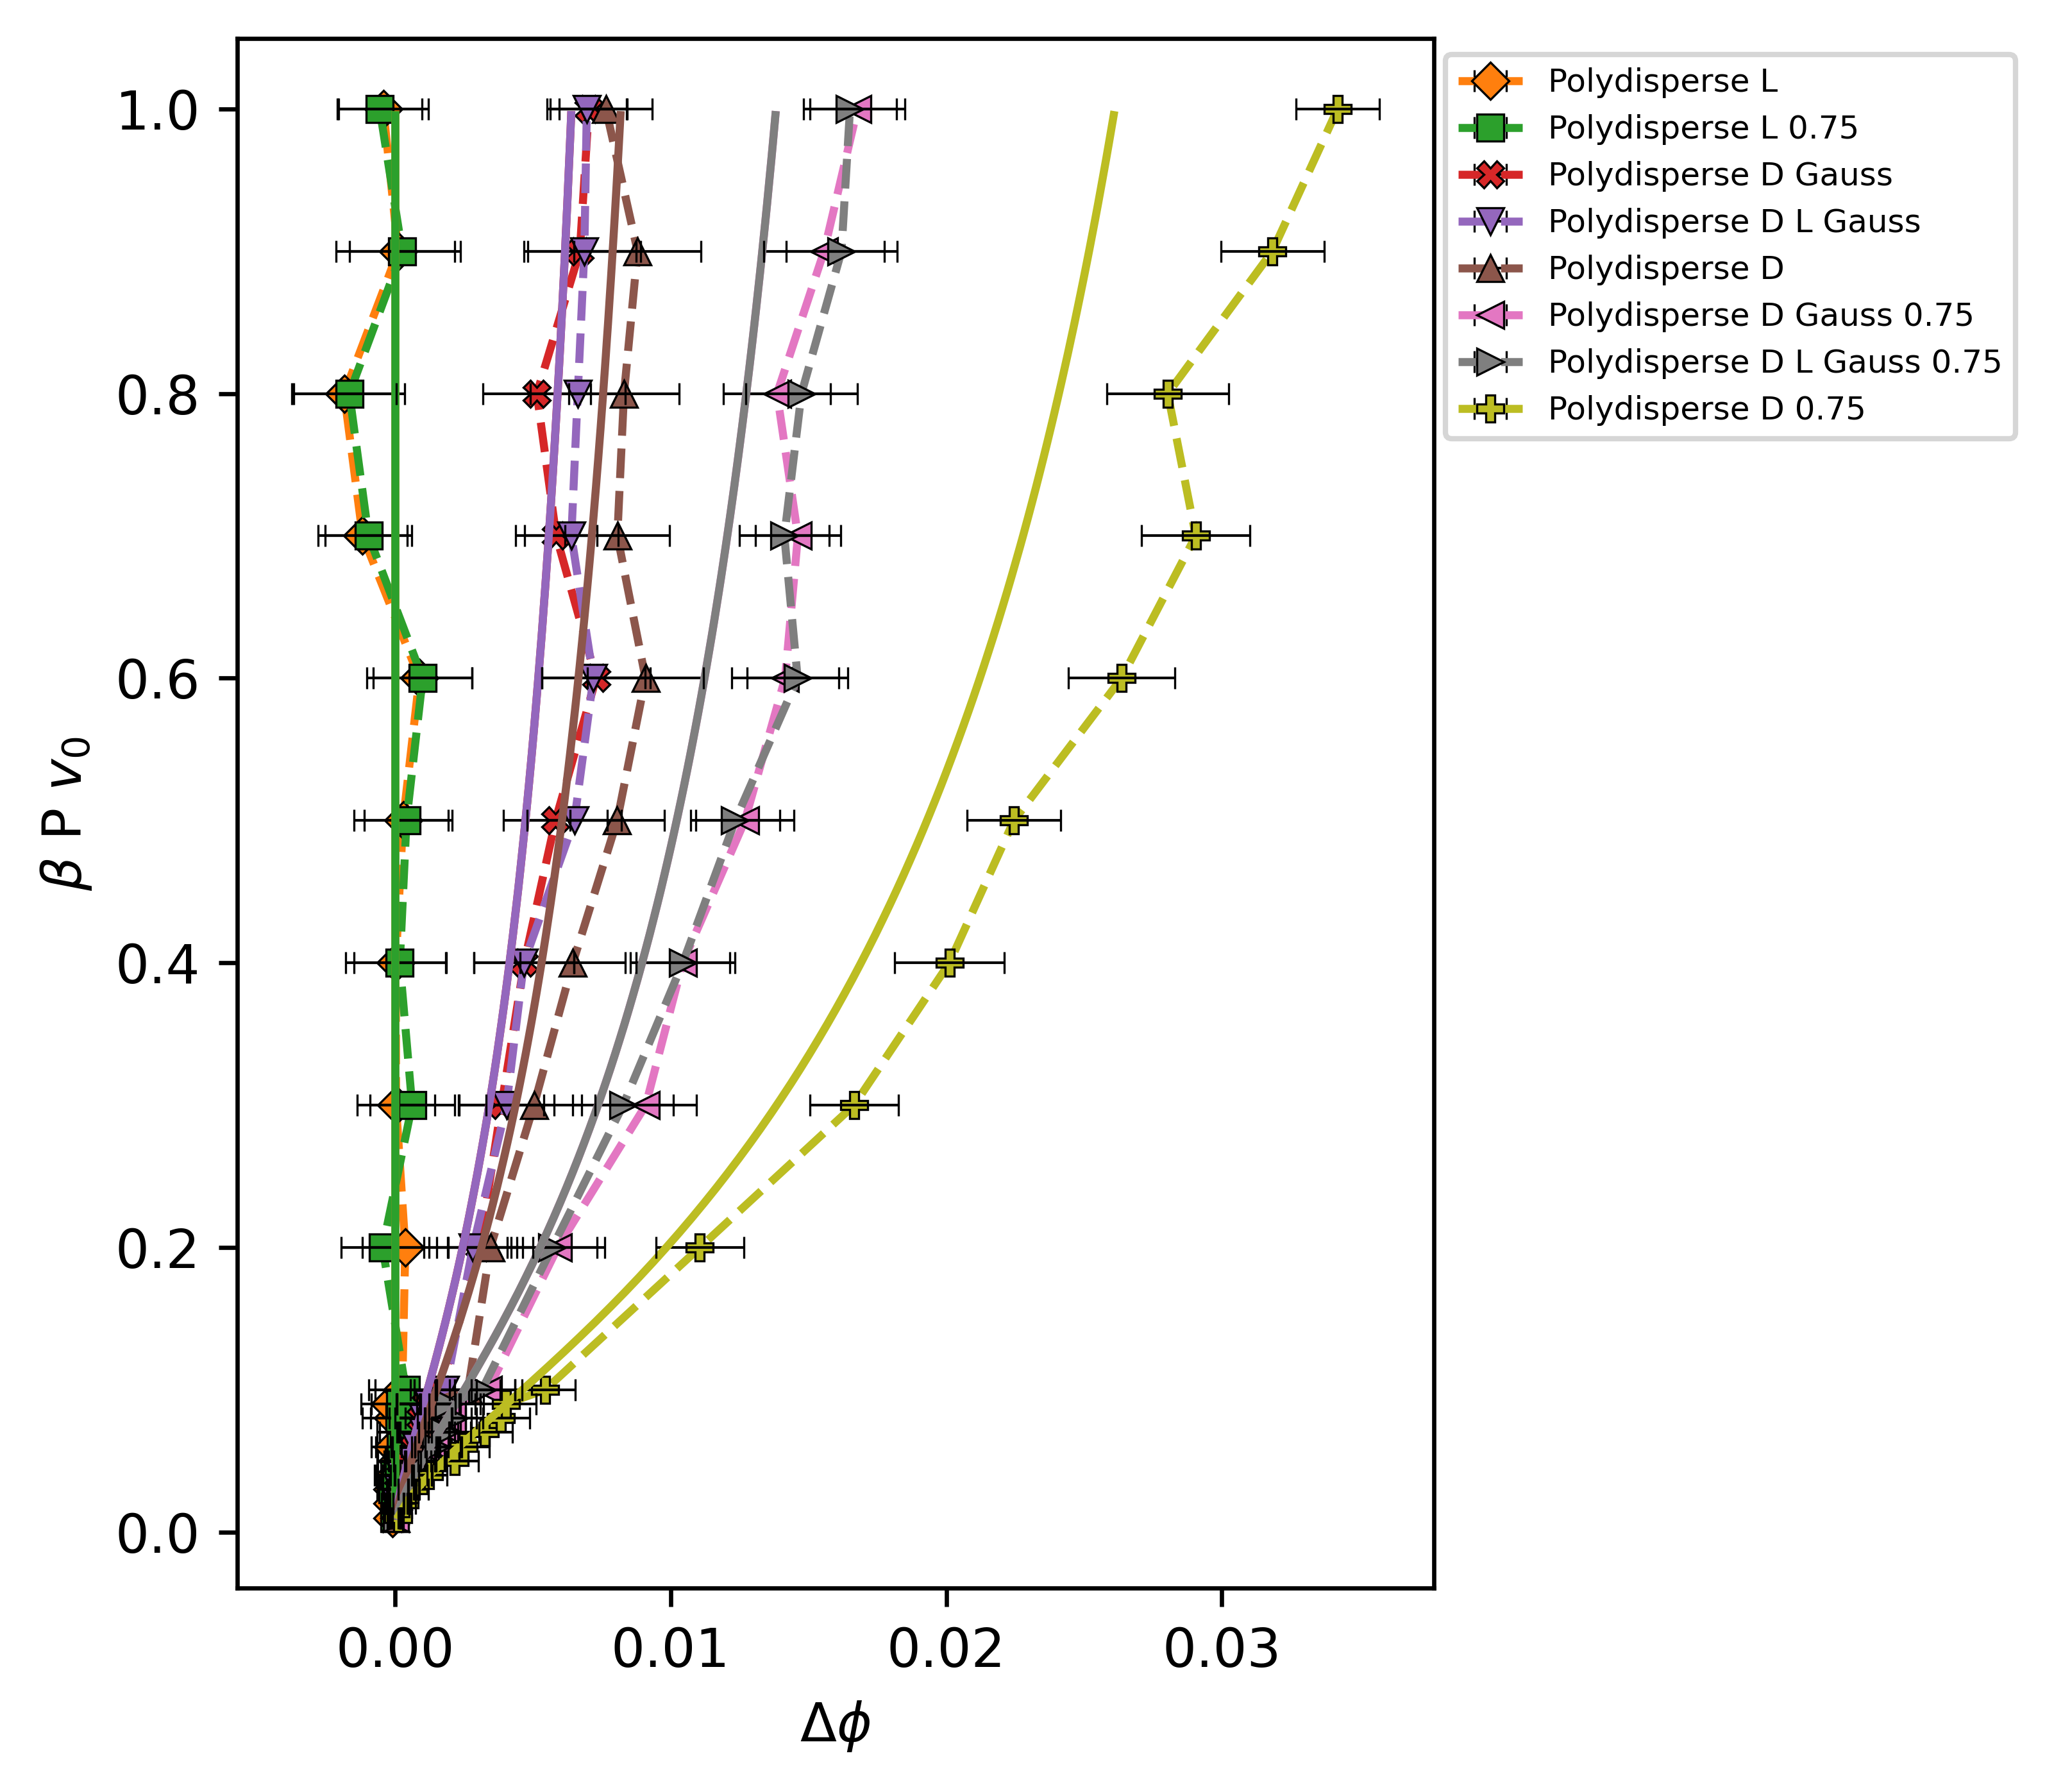
\includegraphics[width=0.45 \columnwidth]{Figures/Deltaphi_P_A1.png}
    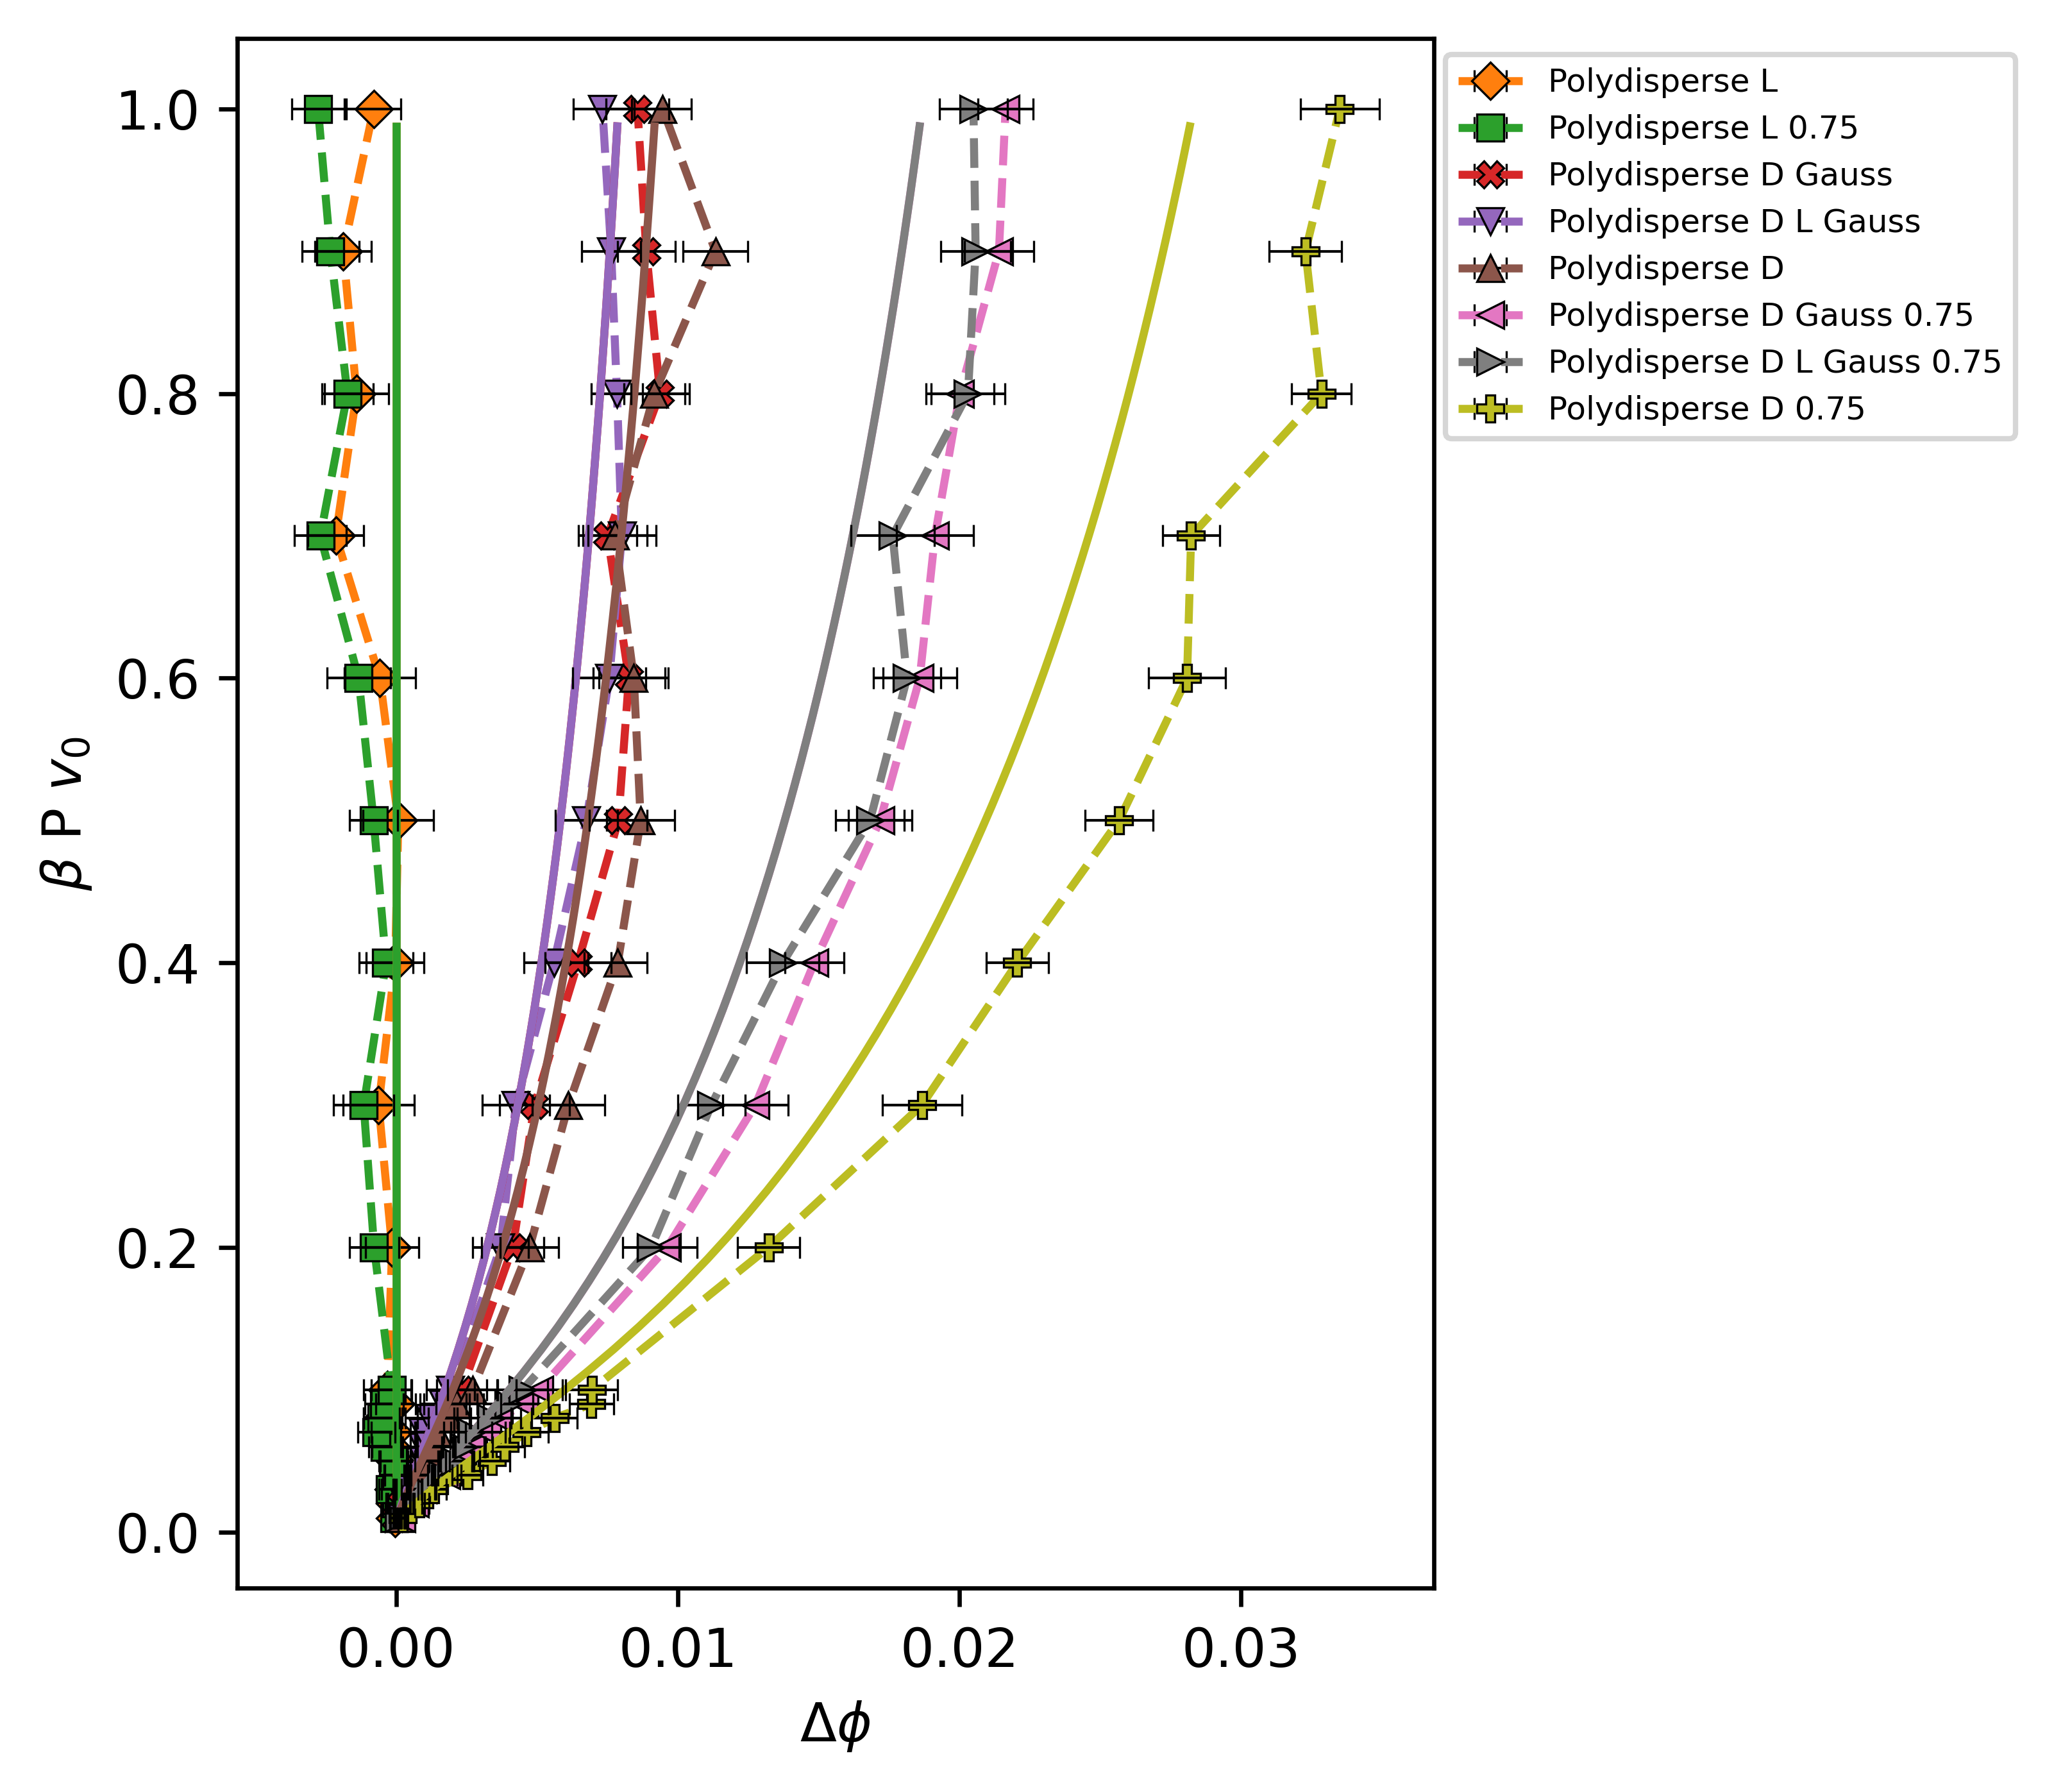
\includegraphics[width=0.45 \columnwidth]{Figures/Deltaphi_P_A5.png}
    \caption{Quantitative theory agreement. Difference between the polydisperse cases and the monodisperse one for the different systems analysed in this work for $A = 1$ (left) and $A = 5$ (right).}
    \label{fig:DeltaP_P}
\end{figure}

This result is on the one hand exciting as it implies that a simple theoretical calculation is able to predict qualitatively and quantitatively EOS in any  polydisperse system if the corresponding monodisperse one is known. Secondly, we can analyse in depth the various contributions to $F$ to assess the reason underlying the independency of the EOS on a polydispersity in $L$, and evict why $D$ plays such a crucial role. As a matter of fact, the main term affecting the theoretical free energy is the ratio between the average excluded volume between all particles in solution, and mean particle volume $v_0$.

We report in table QUISSOTTO  the ratio $\tilde{v}=\overline{v}_{excl}/v_0$ for all of the polydispersities analysed in the system both in $D$ and in $L$. It clearly appears that $\tilde{v}$ is unaffected by any $L$ polydispersity, while all of the different considered polydispersity distributions in $D$ contribute to obtain a different $\tilde{v}$, we can thus conclude that $\tilde{v}=\tilde{v}(D)$. 

\begin{center}
\begin{tabular} { | c | c | }
\hline 
 & Monodisperse \\
 \hline
 $\overline{v_{excl}}$ & a  \\
 \hline
 $v_0$ & d  \\
 \hline
 $\tilde{v}$ & b \\
\hline
\end{tabular}
\end{center}

\section{Conclusions}


We then undergo an in depth analysis separating the $L$ and $D$ contributions to the polydisperse $A$ distribution. 
Interestingly, the change in compressibility of the polydisperse solution with respect to their monodisperse counterparts, is dominated by the  $D$ polydispersity, while even a $100\%$ polydispersity in $L$ does not change the  equation of state obtained for the monodisperse case. To explain such a phenomenon, we studied both global and local properties of the solutions, introducing global and orientational pair distribution functions. Such analyses showed the emergence of a local alignment between the elongated nanoparticles, even in dilute systems. 
%%%
%Qui aggiungiamo il commento sul fatto che sia il volume escluso a dominare - CONTROLLIAMO BENE 
%%%
We show that the more the nanoparticles are elongated, the higher is the local cooperativity in alignment. Moreover the average number of particles that are involved in the local pre-nematic ordering is higher the more anisotropic the particles  are.
Nevertheless such an effect is present both in polydisperse as well as in monodisperse systems. 
To understand why polidispersities in $D$ and $L$ play such a different role on the EOS, we  generalise, to the polydisperse case,  a standard theoretical tool that estimates the equation of state of the solutions through a mean field approach. We use the Parson Lee approximation for estimating the excluded volume effect on the free energy of the system, and analyse the effect of a set of different probability  distributions for $L$ and for $D$ on the equilibrium properties of the solutions. 
Even the theoretical approach shows a strong effect of the compressibility correlated to a polydispersity in $D$, while none of the considered distributions for the polydispersity in $L$ affect the EOS.  We notice that the free volume term is dominated by a $D^3$ contribution, while the strongest contribution arising from $L$ scales as $L^2$. This result seem to indicate that while the presence of anysotropy induce a preferential alignement between particles even at low $\phi$, the strongest effect on compressibility is linked to the excluded volume term. 

%In this paper is analysed the effect of polydispersity onto the low packing fraction phase diagram of functionalisable hard colloidal particles of various anisotropy. 

The paper is structured as follows: in the fist part, we estimate the monodisperse low packing fraction phase diagram for hard spherocylinders with  $A=L/D \in [1,5]$. We then introduce polydispersity on both $L$ and $D$, fixing the average $A$ to be comparable with the monodisperse case. Polydispersity is introduced on $A$, $D$ and $L$, and all contributions to the total polydispersity of the nanoparticles are analysed both globally as well as separately. This analysis demonstrates the predominant role of the polydispersity on $D$ on the equilibrium properties of the solutions, while a polydispersity in $L$ does not seem to have any effect on the packing of the nanoparticles for a given equilibrium pressures. 
We then introduce and generalise the Parson Lee approximation for the equation of state of elongated nanoparticles, to the case in which nanoparticles are polydisperse (generalising the calculation of the excluded volume term in the Excess Pressure to the polydisperse case), and compare the results obtained to the simulation results. Even if Parson Lee approximation is known to well reproduce the phase diagram at intermediate packing fraction, we show that the theoretical predictions at low packing fraction  worsen with increasing $A$, in all considered cases. Nevertheless the theoretical predictions underestimate by only about $10\%$ the worse case scenario. 
At last, we analyse both global and local properties of the solutions by computing the pair distribution functions between all particles, the nematic parameter, and the local orientational pair distribution function. 
While no nematic order is shown by any of the analysed systems in the considered range of the packing fraction, it is possible to appreciate the emergence of a local alignment between the nanoparticles that is enhanced by a higher value of $A$: as soon as $\phi >\phi^*$, local rotational freedom is lost and nanoparticles start aligning one with respect to the other. The local alignement involves a number of particles that is an increasing function of $A$: the more the nanoparticles are anisotropic the higher the number of particles that start aligning locally one with respect to the other.   
From the analysis of the pair distribution function between all particles, it is shown that solutions of slightly anisotropic particles behave similarly to solution of spherical colloids, so that a fluid phase emerges, as $A$ increases, the homogemeous liquid like behaviour is lost.  
The emergence of local alignment between particles is part of the explanation on  why the polydisperse phase diagram for low $\phi$ is almost unaffected by a polydispersity in $L$ and dominated by the polydispersity in $D$: as particles align locally but, no global nematic order arises due to the low concentrations, the ``noise'' introduced by polydispersity on $L$ is not felt by the global properties of the solution, while the one on $D$ affects the average distance between the slightly oriented clusters of particles, thus affecting the global compressibility of the system. 
%%%
% questa va meglio
%%%
This is corroborated by the theoretical approach, that highlights how the excluded volume term - that is dominated bu $D$, affects the EOS



\begin{comment}
Polidispersita in D0.75 puo essere perche e' troppo asimmetrica la distribuzione in A e quindi il sistema e' al limite di una separazione di fase?  secondo me po esse




ISTRUZIONI IMMAGINI:
FAI FIGURE CON MENO TICS E CON FONT PIU GRANDI E SENZA LEGENDA NELLA FIGURA

FAI 
g(r) A=1 A=5
g2(r)  (taglia a 8)



PARSON LEE A=1 A=5 e paragone con simulazioni 

delta phi vs phi  per tutti simulazioni e teo tutte ma A=1, A=5 nel testo altre negli SI
\end{comment}









\begin{comment}
\subsection{References}

The class makes various changes to the way that references are
handled.  The class loads \textsf{natbib}, and also the
appropriate bibliography style.  References can be made using
the normal method; the citation should be placed before any
punctuation, as the class will move it if using a superscript
citation style
\cite{Mena2000,Abernethy2003,Friedman-Hill2003,EuropeanCommission2008}.
The use of \textsf{natbib} allows the use of the various citation
commands of that package: \citeauthor{Abernethy2003} have shown
something, in \citeyear{Cotton1999}, or as given by
Ref.~\citenum{Mena2000}.  Long lists of authors will be
automatically truncated in most article formats, but not in
supplementary information or reviews \cite{Pople2003}. If you
encounter problems with the citation macros, please check that
your copy of \textsf{natbib} is up to date. The demonstration
database file \texttt{achemso-demo.bib} shows how to complete
entries correctly. Notice that ``\latin{et al.}'' is auto-formatted
using the \texttt{\textbackslash latin} command.

Multiple citations to be combined into a list can be given as
a single citation.  This uses the \textsf{mciteplus} package
\cite{Johnson1972,*Arduengo1992,*Eisenstein2005,*Arduengo1994}.
Citations other than the first of the list should be indicated
with a star. If the \textsf{mciteplus} package is not installed,
the standard bibliography tools will still work but starred
references will be ignored. Individual references can be referred
to using \texttt{\textbackslash mciteSubRef}:
``ref.~\mciteSubRef{Eisenstein2005}''.

The class also handles notes to be added to the bibliography.  These
should be given in place in the document \bibnote{This is a note.
The text will be moved the the references section.  The title of the
section will change to ``Notes and References''.}.  As with
citations, the text should be placed before punctuation.  A note is
also generated if a citation has an optional note.  This assumes that
the whole work has already been cited: odd numbering will result if
this is not the case \cite[p.~1]{Cotton1999}.

\subsection{Floats}

New float types are automatically set up by the class file.  The
means graphics are included as follows (Scheme~\ref{sch:example}).  As
illustrated, the float is ``here'' if possible.
\begin{scheme}
  Your scheme graphic would go here: \texttt{.eps} format\\
  for \LaTeX\, or \texttt{.pdf} (or \texttt{.png}) for pdf\LaTeX\\
  \textsc{ChemDraw} files are best saved as \texttt{.eps} files:\\
  these can be scaled without loss of quality, and can be\\
  converted to \texttt{.pdf} files easily using \texttt{eps2pdf}.\\
  %\includegraphics{graphic}
  \caption{An example scheme}
  \label{sch:example}
\end{scheme}

\begin{figure}
  As well as the standard float types \texttt{table}\\
  and \texttt{figure}, the class also recognises\\
  \texttt{scheme}, \texttt{chart} and \texttt{graph}.
  \caption{An example figure}
  \label{fgr:example}
\end{figure}

Charts, figures and schemes do not necessarily have to be labelled or
captioned.  However, tables should always have a title. It is
possible to include a number and label for a graphic without any
title, using an empty argument to the \texttt{\textbackslash caption}
macro.

The use of the different floating environments is not required, but
it is intended to make document preparation easier for authors. In
general, you should place your graphics where they make logical
sense; the production process will move them if needed.

\subsection{Math(s)}

The \textsf{achemso} class does not load any particular additional
support for mathematics.  If packages such as \textsf{amsmath} are
required, they should be loaded in the preamble.  However,
the basic \LaTeX\ math(s) input should work correctly without
this.  Some inline material \( y = mx + c \) or $ 1 + 1 = 2 $
followed by some display. \[ A = \pi r^2 \]

It is possible to label equations in the usual way (Eq.~\ref{eqn:example}).
\begin{equation}
  \frac{\mathrm{d}}{\mathrm{d}x} \, r^2 = 2r \label{eqn:example}
\end{equation}
This can also be used to have equations containing graphical
content. To align the equation number with the middle of the graphic,
rather than the bottom, a minipage may be used.
\begin{equation}
  \begin{minipage}[c]{0.80\linewidth}
    \centering
    As illustrated here, the width of \\
    the minipage needs to allow some  \\
    space for the number to fit in to.
    %\includegraphics{graphic}
  \end{minipage}
  \label{eqn:graphic}
\end{equation}

\section{Experimental}

The usual experimental details should appear here.  This could
include a table, which can be referenced as Table~\ref{tbl:example}.
Notice that the caption is positioned at the top of the table.
\begin{table}
  \caption{An example table}
  \label{tbl:example}
  \begin{tabular}{ll}
    \hline
    Header one  & Header two  \\
    \hline
    Entry one   & Entry two   \\
    Entry three & Entry four  \\
    Entry five  & Entry five  \\
    Entry seven & Entry eight \\
    \hline
  \end{tabular}
\end{table}

Adding notes to tables can be complicated.  Perhaps the easiest
method is to generate these using the basic
\texttt{\textbackslash textsuperscript} and
\texttt{\textbackslash emph} macros, as illustrated (Table~\ref{tbl:notes}).
\begin{table}
  \caption{A table with notes}
  \label{tbl:notes}
  \begin{tabular}{ll}
    \hline
    Header one                            & Header two \\
    \hline
    Entry one\textsuperscript{\emph{a}}   & Entry two  \\
    Entry three\textsuperscript{\emph{b}} & Entry four \\
    \hline
  \end{tabular}

  \textsuperscript{\emph{a}} Some text;
  \textsuperscript{\emph{b}} Some more text.
\end{table}

The example file also loads the optional \textsf{mhchem} package, so
that formulas are easy to input: \texttt{\textbackslash ce\{H2SO4\}}
gives \ce{H2SO4}.  See the use in the bibliography file (when using
titles in the references section).

The use of new commands should be limited to simple things which will
not interfere with the production process.  For example,
\texttt{\textbackslash mycommand} has been defined in this example,
to give italic, mono-spaced text: \mycommand{some text}.

\section{Extra information when writing JACS Communications}

When producing communications for \emph{J.~Am.\ Chem.\ Soc.}, the
class will automatically lay the text out in the style of the
journal. This gives a guide to the length of text that can be
accommodated in such a publication. There are some points to bear in
mind when preparing a JACS Communication in this way.  The layout
produced here is a \emph{model} for the published result, and the
outcome should be taken as a \emph{guide} to the final length. The
spacing and sizing of graphical content is an area where there is
some flexibility in the process.  You should not worry about the
space before and after graphics, which is set to give a guide to the
published size. This is very dependant on the final published layout.

You should be able to use the same source to produce a JACS
Communication and a normal article.  For example, this demonstration
file will work with both \texttt{type=article} and
\texttt{type=communication}. Sections and any abstract are
automatically ignored, although you will get warnings to this effect.
\end{comment}




%%%%%%%%%%%%%%%%%%%%%%%%%%%%%%%%%%%%%%%%%%%%%%%%%%%%%%%%%%%%%%%%%%%%%
%% The "Acknowledgement" section can be given in all manuscript
%% classes.  This should be given within the "acknowledgement"
%% environment, which will make the correct section or running title.
%%%%%%%%%%%%%%%%%%%%%%%%%%%%%%%%%%%%%%%%%%%%%%%%%%%%%%%%%%%%%%%%%%%%%
\begin{acknowledgement}

The Grant of Excellence Departments, MIUR-Italy (ARTICOLO 1, COMMI 314 - 337 LEGGE 232/2016) is gratefully acknowledged.

\end{acknowledgement}

%%%%%%%%%%%%%%%%%%%%%%%%%%%%%%%%%%%%%%%%%%%%%%%%%%%%%%%%%%%%%%%%%%%%%
%% The same is true for Supporting Information, which should use the
%% suppinfo environment.
%%%%%%%%%%%%%%%%%%%%%%%%%%%%%%%%%%%%%%%%%%%%%%%%%%%%%%%%%%%%%%%%%%%%%

\begin{comment}
\begin{suppinfo}

This will usually read something like: ``Experimental procedures and
characterization data for all new compounds. The class will
automatically add a sentence pointing to the information on-line:

\end{suppinfo}
\end{comment}




%%%%%%%%%%%%%%%%%%%%%%%%%%%%%%%%%%%%%%%%%%%%%%%%%%%%%%%%%%%%%%%%%%%%%
%% The appropriate \bibliography command should be placed here.
%% Notice that the class file automatically sets \bibliographystyle
%% and also names the section correctly.
%%%%%%%%%%%%%%%%%%%%%%%%%%%%%%%%%%%%%%%%%%%%%%%%%%%%%%%%%%%%%%%%%%%%%
\bibliography{polyhsc}

\end{document}
